%% Load document class fithesis2
%% {10pt, 11pt, 12pt}
%% {draft, final}
%% {oneside, twoside}
%% {onecolumn, twocolumn}
\documentclass[11pt,final,twoside]{fithesis2}

%% Basic packages
\usepackage[czech]{babel}
\usepackage{cmap}
\usepackage[T1]{fontenc}
\usepackage{lmodern}
\usepackage[utf8]{inputenc}
\usepackage{graphicx}

%% Additional packages for colors, advanced
%% formatting options, etc.
\usepackage{color}
\usepackage{microtype}
\usepackage{url}
\usepackage{cslatexquotes}
\usepackage{fancyvrb}
\usepackage[small,bf]{caption}
\usepackage[plainpages=false,pdfpagelabels,unicode]{hyperref}
\usepackage[all]{hypcap}
\usepackage{listings}
\usepackage{array}
\usepackage{color}

\definecolor{mygreen}{rgb}{0,0.6,0}
\definecolor{mygray}{rgb}{0.5,0.5,0.5}
\definecolor{mymauve}{rgb}{0,0,0}

\lstset{ %
   backgroundcolor=\color{white},   % choose the background color; you must add \usepackage{color} or \usepackage{xcolor}
   basicstyle=\footnotesize,        % the size of the fonts that are used for the code
   breakatwhitespace=false,         % sets if automatic breaks should only happen at whitespace
   breaklines=false,                 % sets automatic line breaking
   captionpos=b,                    % sets the caption-position to bottom
   commentstyle=\color{mygreen},    % comment style
   deletekeywords={...},            % if you want to delete keywords from the given language
   escapeinside={\%*}{*)},          % if you want to add LaTeX within your code
   extendedchars=true,              % lets you use non-ASCII characters; for 8-bits encodings only, does not work with UTF-8
   frame=single,                    % adds a frame around the code
   keepspaces=true,                 % keeps spaces in text, useful for keeping indentation of code (possibly needs columns=flexible)
   keywordstyle=\color{blue},       % keyword style
   language=Octave,                 % the language of the code
   morekeywords={*,...},            % if you want to add more keywords to the set
   numbers=left,                    % where to put the line-numbers; possible values are (none, left, right)
   numbersep=5pt,                   % how far the line-numbers are from the code
   numberstyle=\tiny\color{mygray}, % the style that is used for the line-numbers
   rulecolor=\color{black},         % if not set, the frame-color may be changed on line-breaks within not-black text (e.g. comments (green here))
   showspaces=false,                % show spaces everywhere adding particular underscores; it overrides 'showstringspaces'
   showstringspaces=false,          % underline spaces within strings only
   showtabs=false,                  % show tabs within strings adding particular underscores
   stepnumber=1,                    % the step between two line-numbers. If it's 1, each line will be numbered
   stringstyle=\color{mymauve},     % string literal style
   tabsize=2,                       % sets default tabsize to 2 spaces
   title=\lstname                   % show the filename of files included with \lstinputlisting; also try caption instead of title
}

\renewcommand\lstlistingname{Kód}

\newcommand*{\captionsource}[2]{%
  \caption[{#1}]{%
    #1%
    \\\hspace{\linewidth}%
    \textbf{Zdroj:} #2%
  }%
}

%% Fix long URLs in DVIs
\usepackage{ifpdf}

\ifpdf
\else
  \usepackage{breakurl}
\fi

%% Packages used to generate various lists
\usepackage{makeidx}
\makeindex

\usepackage[xindy]{glossaries}
\makeglossary

%% Use STAR and CIRCLE signs for nested
%% itemized lists
\renewcommand{\labelitemii}{$\star$}
\renewcommand{\labelitemiii}{$\circ$}

%% Title page information
\thesistitle{Komponenta distribuce a správy klíčů pro bezdrátové sensorové sítě}
\thesissubtitle{bakalářská práce}
\thesisstudent{Lukáš Němec}
\thesiswoman{false} %% Important when using Slovak or Czech lang
\thesisfaculty{fi}  %% {fi, eco, law, sci, fsps, phil, ped, med, fss}
\thesislang{cs}     %% {en, sk, cs}
\thesisyear{jaro 2014}
\thesisadvisor{RNDr. Petr Švenda, Ph.D.}

%% Beginning of the document
\begin{document}

%% Front page with a logo and basic thesis information
\FrontMatter
\ThesisTitlePage

%% Thesis declaration (required)
\begin{ThesisDeclaration}
  \DeclarationText
  \AdvisorName
\end{ThesisDeclaration}

%% Thanks (optional)
\begin{ThesisThanks}
TODO

Tato práce vznikla na základě projektu VG20102014031, který je součástí
Programu bezpečnostního výzkumu České republiky v letech 2010 - 2015
(BVII/2 - VS).
\end{ThesisThanks}

%% Abstract (required)
\begin{ThesisAbstract}
TODO
\end{ThesisAbstract}

%% Keywords (required)
\begin{ThesisKeyWords}
TODO
\end{ThesisKeyWords}

%% Beginning of the thesis itself
\MainMatter

%% TOC (required)
\tableofcontents

%% Thesis text structured using
%% chapters, sections, subsections, etc.
\chapter{Úvod}
Bezdrátová sensorová síť je složená z velkého množství malých autonomních zařízení, které spolu navzájem komunikují přes rádiové spojení. Každé zařízení, nazývané sensorový uzel, je napájené pomocí
baterií a je vybavené potřebnými sensory pro monitorování okolí. Pokroky v oblasti vývoje a výroby integrovaných obvodů vedly v poslední době k dramatické redukci jejich velikosti, spotřeby elektrické 
energie a ceny, což nám umožňuje využívat sensorové sítě v široké škále aplikací. Typický scénář nasazení sensorové sítě je náhodné rozmístění stovek až tisíců uzlů a následný sběr dat pomocí jednotlivých 
sensorů. Jako příklady oborů, kde mohou bezdrátové sensorové sítě nalézt uplatnění, lze uvést například armádu, zdravotnictví, zemědělství a další. Konkrétně je možné zmínit projekt SmartDust 
\cite{Kahn1999}, nebo projekt sledování sopečné aktivity \cite{Werner-Allen2006}. 

V mnohých případy uplatnění bezdrátových sensorových sítí je však kritické zabezpečení informací předávaných mezi jednotlivými uzly. Především se snažíme o zajištění důvěrnosti a autenticity jednotlivých 
zpráv. Důvěrnost je potřeba zajistit v případě monitorování citlivých (zdravotní stav osoby, pohyb osob v monitorované oblasti), nebo jinak cenných informací. Taktéž můžeme mít zájem, aby vlastník sítě měl 
možnost informace získané sensory zpeněžit, což by nebylo možné, pokud by byly veřejně dostupné. V případě autenticity jednotlivých zpráv je podstatné, aby pro útočníka nebylo možné do sítě přidávat vlastní 
uzly nebo jiným způsobem modifikovat komunikaci. Zcela jistě je nežádoucí, aby sensory, určené pro varování před přírodními katastrofami, vyvolávaly falešné poplachy. Díky aktuální situaci, kdy vývoj 
bezdrátových sítí je stále v raném stádiu, máme jedinečnou možnost sítě budovat bezpečné již od počátku. Díky tomu se můžeme vyhnout dodatečnému přidávání bezpečnostních opatření a tím předejít 
budoucím problémům.

Pro sensorové uzly je v~současné době velmi rozšířený operační systém TinyOS \cite{Levis2005}, který vznikl na univerzitě v~Berkeley a v~současné době je vyvíjen jako open-source projekt.  Tento systém 
zabezpečuje jak zasílání a příjem zpráv mezi jednotlivými uzly, tak zároveň obsluhu sensorů na jednotlivých uzlech i vše ostatní nezbytné pro fungování sensorové sítě. Systém se vyskytuje na několika 
hardwarových platformách, mezi nejběžnější patří TelosB a MICAz \cite{Inc.}\cite{MemsicInc.}. TinyOS však obsahuje zranitelná místa, která mohou být využita potencionálním útočníkem \cite{Drexler2010} a pro 
reálnou použitelnost tohoto systému je zapotřebí tyto mezery v~zabezpečení odstranit. Práce samotná se tedy zabývá bezpečností v bezdrátových sensorových sítí, konkrétně problematikou výměny klíčů.

Cílem práce je vybrat vhodné schéma pro distribuci a správu klíčů v bezdrátové sensorové síti, toto schéma implementovat a začlenit do vyvíjené platformy ProtectLayer \cite{Svenda2014a}, která slouží pro 
ochranu komunikace v bezdrátových sensorových sítích, a poté vyhodnotit výsledky z experimentálního provozu této platformy. Struktura práce samotné je následující:

\begin {itemize}
\item První kapitola obsahuje popis a hodnocení již existujících schémat pro distribuci a správu klíčů v bezdrátových sítích pro platformu TinyOS. Nejdříve jsou uvedena klasická řešení problému distribuce 
klíčů a zároveň odůvodnění, proč tyto nejsou vhodné pro použití v bezdrátových sensorových sítích. Následuje šest vybraných schémat pro distribuci klíčů, kdy u každého je uveden krátký popis principu 
fungování a následně hodnocení schématu z hlediska možného použití ve vyvíjené komponentě. 

\item Druhá kapitola se zabývá samotnou implementací vybraného schématu pro platformu TelosB v rámci vyvíjené komponenty, tedy nejdříve je popsán samotný systém TinyOS, včetně specifických vlastností tohoto 
systému. Následuje popis vybraného schématu, se zaměřením na skutečnosti, které byly rozhodující při výběru. Poslední část této kapitoly se zabývá implementací samotnou, jsou zde popsány změny v implementaci 
oproti původnímu schématu a popis důležitých vlastností jak hlavní komponenty pro správu klíčů, tak podpůrných komponent zabezpečujících kryptografické funkce. 

\item V poslední kapitole je popsán experiment, který proběh v únoru 2014, jehož cílem bylo ověření funkčnosti celé vyvíjené platformy. V kapitole je tedy popsán scénář samotného experimentu, poté nástroje 
které byly použity k vyhodnocení. Na konec jsou uvedeny výsledky samotné včetně doplňujících komentářů k nim. 
\end{itemize}



\chapter{Existující implementace pro distribuci a správu klíčů}
Mechanismus bezpečného ustanovení klíčů pro komunikaci v bezdrátové sensorové síti tvoří jeden ze základních předpokladů 
pro bezpečné a spolehlivé fungování sítě jako celku. Na zabezpečenou komunikaci například spoléhá protokol pro ustanovení cest v síti (je třeba k ustanovení cesty v síty využít
pouze autentizované uzly, nikoliv uzly útočníka které mohou nabízet výhodnější cestu), protokoly pro společné výpočty v síti (uzel kontroluje hodnoty naměřené svými sensory oproti
hodnotám naměřeným na okolních uzlech, a detekuje tak možné chyby) a případně protokoly pro detekci a reakci na provedený útok \cite{Alcaraz2012}.

Přitom co se možných řešení týká, jsme zde limitování mnohými rozdíly oproti sítím v klasické podobě. Mezi nejvýznamnější rozdíly například
patří omezené možnosti napájení (jednotlivé uzly mají většinou vlastní baterii a snahou je interval nutných výměn prodloužit co nejvíce), 
většinu spojení nemůžeme považovat za trvalé (topologie sítě se může měnit, případně uzly z důvodu úspory energie komunikují pouze v určitých 
intervalech) a musíme počítat s faktem, že hardware uzlu, především z důvodu ceny, nemá žádnou ochranu proti násilnému získání obsahu paměti uzlu, 
tedy i případných kryptografických klíčů v paměti obsažených. Následují tedy jednotlivé klasické možnosti správy klíčů s odůvodněním proč nejsou pro 
použití v rámci sensorové sítě vhodné.

\section{Klasické přístupy k řešení problému distribuce klíčů}
\subsection{Jeden sdílený klíč (master key)} Řešení pomocí jednoho sdíleného klíče, který zabezpečuje veškerou komunikaci je sice nejjednodušší a 
nejméně náročné co se implementace týká, nicméně tím výčet výhod tohoto řešení končí a následují nevýhody, které převažují. Tou nejdůležitější 
je problém v případě, že se útočníkovi podaří získat jediný uzel z celé sítě, tedy získá sdílený klíč pro komunikaci v rámci celé sítě. Následně 
má jednak možnost dešifrovat všechny zprávy zaslané v síti a jednak má možnost vysílat vlastní zprávy bez možnosti detekce.

\subsection{Párové klíče (Pairwise keys)} Zde již je kompromitování komunikace v celé síti vyřešeno pomocí separátních klíčů pro každý uzel, 
tedy útočník se získáním uzlu získá pouze zprávy směřující k tomuto uzlu, případně možnost vydávat se za tento uzel, nicméně toto řešení 
obsahuje jiný problém. V případě skutečně rozsáhlé sítě (tisíce až sta tisíce uzlů) není technicky možné, aby paměť uzlu obsahovala natolik 
velké množství klíčů, minimálně hardware který je v současné době dostupný pro stavbu sensorových sítí toto neumožňuje\footnote{pokud uvažujeme 
AES \cite{Daemen1999} klíč o velikosti 128 bitů a 1000 uložených klíčů v paměti uzlu, dostáváme celkem 16 KB dat, které je potřeba uložit do paměti uzlu. 
Pokud uvažujeme například platformu TelosB \cite{MemsicInc.}, zde sice máme k dispozici 1MB paměti určené k ukládání dat, ale RAM paměť uzlu je pouze 10KB. 
A to nepočítáme s dalšími daty, které se kterými je potřeba pracovat, například naměřené hodnoty sensorů či další data aplikace. Celý problém je navíc umocněn tím, že
primárním cílem není zabezpečená komunikace, ale sběr dat pomocí sensorů, tedy kryptografická data by měla zabírat pouze zlomek celkové paměťové kapacity uzlu.}.
Hlavní slabinou této varianty je tedy velmi velká paměťová náročnost a obtížná škálovatelnost pro rozsáhlejší sítě. 

\subsection{Asymetrická kryptografie} Při použití asymetrické kryptografie narážíme na problém ve omezeném výpočetním výkonu jednotlivých uzlů, 
které jsou aktuálně schopné provádět pouze podmnožinu operací potřebných k bezpečnému fungování asymetrické kryptografie tak jak ji známe.
Na druhou stranu existují implementace asymetrické kryptografie pro použití v rámci bezdrátových sensorových sítí \cite{Watro2004}, nicméně 
tyto nejsou určeny pro komunikaci mezi jednotlivými uzly navzájem, ale spíše pro zasílání informací od sensorů k třetí straně. 
Navíc při použití veřejných klíčů vyvstává problém s jejich revokací a opět je zde problém, že klíč z uzlu, který získá útočník může být použit 
na kterémkoliv místě v síti.

Celkově zhodnoceno, většina známých klasických přístupů není vhodná pro řešení správy klíčů v bezdrátové sensorové síti, je tedy na místě hledat alternativní řešení,
která již budou brát v úvahu všechna omezení těchto sítí a využijí vlastnosti bezdrátových sensorových sítí ve svůj prospěch.

\section{Pravděpodobnostní rozdělení klíčů (Eschenauer a Gligor)} \label{sec:Eschenauer}
Návrh pravděpodobnostního rozdělení klíčů \cite{Eschenauer2002} řeší elegantním způsobem problém přílišné paměťové náročnosti při použití párových klíčů a je 
založen na narozeninovém paradoxu díky kterému můžeme vypočítat pravděpodobnost s jakou dva uzly sdílejí stejný klíč. 
Celkově se schéma skládá ze tří fází, první obsahuje predistribuci vybraných klíčů, druhá nalezení sdílených klíčů a třetí řeší nalezení cest v síti.

\subsection{Popis fungování schématu}
Samotná první fáze se skládá z několika kroků, nejdříve je vygenerována velká množina $P$ klíčů, z těchto je následně náhodně vybráno $k$ klíčů pro každý
uzel. Počet $k$ vybraných klíčů je určen celkovým počtem uzlů a požadovanou pravděpodobností sdíleného klíče mezi sousedními uzly. Celá tato první fáze 
probíhá před samotným rozmístěním uzlů. Následuje druhá fáze, která nastává ve fázi inicializace sítě, kdy jednotlivé uzly zjistí své sousedy v dosahu 
rádiové komunikace a zjistí, se kterými sdílí klíč. Nejednoduší cesta, jak toto provést je, že každý uzel odešle všem ostatním ve svém okolí seznam jím 
vlastněných klíčů. Seznam identifikátorů jednotlivých klíčů není potřeba považovat za citlivou informaci, proto tento postup postačuje. V případě potřeby 
jej ale lze nahradit tak, že uzel odešle výzvy zašifrované pomocí všech klíčů, které vlastní. pokud se příjemci podaří výzvu úspěšně dešifrovat, pak
uzly mají společný klíč. Následuje ustanovení cest v síti, kdy je vyhledána cesta mezi uzly sítě, které nevlastní společný klíč, nicméně je možné je propojit 
komunikací přes ostatní uzly, které klíč sdílejí. Touto cestou je následně vyměněn nový klíč pro přímé spojení. 

Při následné komunikaci je v případě potřeby možné celý proces nalezení sdílených klíčů a cest v síti spustit znovu, například v případě získání části klíčů útočníkem
je možné tyto klíče revokovat (zasláním zprávy z centrálního uzlu) a cesty ustanovit znovu bez použití těchto klíčů. Stejný proces může být inicializován i samotným uzlem
a to v případě potřeby použití nových klíčů pro spojení. 

\subsection{Vhodnost použití}
Celé schéma si při své jednoduchosti zachovává velmi dobrou funkčnost a v případě potřeby komunikace pouze mezi uzly samotnými se pravděpodobně jedná o nejvýhodnější
variantu řešení a to především pro případy, kdy je rozmístění jednotlivých uzlů náhodné a nemůžeme počítat s předem určenou topologií sítě. Schéma je taktéž velmi dobře kombinovatelné
s dalšími jednoduchými způsoby komunikace a tedy rozšířitelné o případnou další funkcionalitu. Z hlediska implementace a náročnosti na hardware jednotlivých uzlů schéma
splňuje všechny požadavky, nicméně schéma tak jak je nevyhovuje pro použití v rámci vyvíjené komponenty především z důvodu nedostatečné funkcionality. Schéma sice zajistí ustanovení
a správu komunikace mezi uzly samotnými, ale neřeší jakékoliv návazné problémy, jako například hromadné posílání zpráv z centrálního uzlu a vyžadovalo by příliš mnoho modifikací oproti 
původnímu návrhu a proto nebylo vybráno.

\section{Upravené pravděpodobnostní rozdělení (Chan, Perrig a Song)} \label{sec:Chan}
Návrh dvou možnosti rozšíření \cite{Perrig2003} předchozího schématu \cite{Eschenauer2002} tak, aby bylo odolnější vůči možným útokům a aby síť měla možnost znovu zabezpečit spojení, jehož
klíč byl prozrazen. Obě části počítají se stejnými podmínkami jako předchozí, tedy nahrání množiny klíčů na jednotlivé uzly s tím, že jednotlivé klíče jsou náhodně vybrány 
z větší množiny všech generovaných klíčů.

\subsection{Q-kompozitní klíč (q-composite key)}
Oproti původnímu návrhu, zde je ustanovena hodnota $q$, která vyjadřuje počet sdílených klíčů, které musí sousední uzly sdílet, aby bylo možné ustanovit spojení. Při původní variantě 
je hodnota $q$ rovna jedné a tedy není potřeba se jí zabývat. Zde ovšem hraje důležitou roli z hlediska zvýšení zabezpečení sítě. Sousední uzly opět vysíláním identifikátorů klíčů které vlastní
zjistí, se kterými sousedy sdílejí alespoň $q$ klíčů a s těmito zahájí komunikaci. Předpokládejme tedy, že dva uzly sdílejí $q'$ klíčů $k_1, k_2 \dots k_{q'}$ ($q' \ge q$) a existenci hashovací funkce $H$, 
společný klíč $k$ pro následující komunikaci mezi uzly je tedy ustanoven následovně $k=H(k_1 || k_2 || \dots || k_{q'})$ s tím, že je zabezpečené stejné pořadí klíčů, například podle původního
pořadí v jakém byly generovány. 

Schéma zachovává původní princip nalezení cesty mezi uzly, které na začátku nevlastní potřebný počet společných klíčů a taktéž původní princip revokace klíčů pomocí zaslání zprávy z 
centrálního uzlu. Celkově zlepšení poskytuje zvýšenou ochranu proti útokům malého rozsahu za cenu snížení odolnosti proti útokům většího rozsahu. Zde je možné konstatovat, že se jedná 
o žádoucí vlastnosti, jelikož malé útoky je těžké zaznamenat (malé procento nefunkčních uzlů může být běžný jev), zatímco útoky na výrazně větší množství uzlů již pravděpodobně zaznamenány budou a 
bude tedy možné provést patřičná protiopatření. 

\subsection{Vícecestné obnovením spojení (multipath)}
Druhý návrh \cite{Svenda2009} se zabývá obnovením spojení, jehož klíč byl prozrazen, nicméně uzly samotné zůstaly útokem nedotčeny. K této situaci například dojde, pokud je klíč používaný pro komunikaci mezi
uzly $A$ a $B$ uložen v paměti uzlu $C$ a útočník získá klíče na uložené na uzlu $C$. Obnovení komunikačního klíče je provedeno přes více nezávislých cest, konkrétně uzly $A$ a $B$ zjistí společné sousedy
přes které se mohou spojit tak, že délka cesty je kratší než předem stanovená maximální hodnota přeskoků. Pokud tedy existuje $j$ cest spojujících tyto dva uzly, pak uzel $A$ pošle po každé cestě náhodně 
generovanou hodnotu $v$, celkově tedy pošle hodnoty $v_1, v_2, \dots v_j$. Na uzlu $B$ je nová hodnota klíče spočítána z původní hodnoty následovně $k' = k \oplus v_1 \oplus v_2 \oplus \dots \oplus v_j$

Tato metoda celkově způsobí znatelné zatížení sítě, především pro větší dovolený počet přeskoků. Pokud však dovolíme pouze malý počet přeskoků (například dva) zaznamenáme zlepšení v odolnosti proti 
případným útokům. Především síť dokáže obnovit spojení, která jsou přerušena vyzrazením použitého klíče.

\subsection{Vhodnost použití}
Autoři nedoporučují oba navržené přístupy kombinovat, protože při použití obou dojde ke zkombinovaní negativních dopadů obou, tedy zmenšení celkového počtu klíčů aby bylo dostatečné množství shodných
klíčů mezi jednotlivými uzly a k nárůstu komunikace z důvodu obnovování jednotlivých spojení. 

Oba návrhy jsou zajímavým řešením, které zlepší zabezpečení sítě oproti původní variantě pravděpodobnostního rozdělení klíčů. Varianty se liší způsobem, kterým tohoto zlepšení dosáhnou, q-composite 
varianta posiluje bezpečnost před samotným útokem a tedy odolnost vůči útoku, zatímco multipath poskytuje řešení pro případ úspěšného útoku a nabízí možnost jak minimalizovat škody útokem způsobené.
Co se vhodnosti použití na vyvíjené komponentě týká, opět jsou splněny požadavky kladené omezeným výkonem jednotlivých uzlů, nicméně i přes přidanou funkcionalitu (především ve 
variantě multipath) neobsahuje schéma všechny požadované vlastnosti. Především se nezabývá zabezpečením oboustranné komunikace s centrálním uzlem. Tedy použití by bylo vhodné pouze v kombinaci 
s jiným přístupem. Z tohoto důvodu tedy schéma nebylo vybráno. 


\section{Blomovo pravděpodobnostní rozdělení (Du, Deng, Han a Varshney)}
Zajímavý návrh \cite{Du2005} koncepčně vycházející ze schématu původně navrženého Blomem \cite{Blom1985}, ale rozšiřující jej o pravděpodobnostní rozdělení klíčů \ref{sec:Eschenauer}.
Díky tomu získáváme schéma pro distribuci klíčů vhodné pro použití v bezdrátových sensorových sítích. Oproti předchozím variantám návrh celkově zvyšuje odolnost sítě vůči 
útočníkovi a to za cenu vyšší výpočetní náročnosti, nicméně tato zůstává na rozumné míře (tedy stále výrazně menší než u asymetrické kryptografie). 

\subsection{Původní Blomovo schéma}
Blom \cite{Blom1985} se zabývá řešením problému distribuce klíčů v klasické síti, především s ohledem na velký počet uživatelů a tedy nepraktičnost případně až nemožnost ukládat všechny klíče u uživatele.
Namísto toho navrhuje doručit každému uživateli relativně malé množství dat ze kterého dokáže všechny potřebné klíče odvodit. Schéma je konstruováno tak, aby každá dvojice uživatelů z celkového počtu $n$
dokázala odvodit společný klíč a to pouze při uložení $\lambda + 1$ klíčů, kde $\lambda \ll n$. Co se bezpečnosti týká, dokud není počet kompromitovaných uživatelů (jejich klíčů) vyšší než hodnota 
$\lambda$, pak můžeme všechna spojení považovat za bezpečná. V okamžiku kdy je hodnota $\lambda$ překročena, získává útočník přístup k veškeré komunikaci v síti. 

Schéma je založené na násobení matic, konkrétně proces ustanovení klíčů probíhá následovně: 
nejdříve je zkonstruována matice $G$ o rozměru $(\lambda + 1) \times n$ nad konečným tělesem $GF(q)$, kde sloupce matice $G$ jsou lineárně nezávislé a $q > n$.
Tato matice je veřejně známou informací a každý účastník, včetně útočníka, může znát její obsah. Následuje zkonstruování symetrické matice $D$ s rozměrem $(\lambda + 1) \times (\lambda + 1) $, 
opět nad konečným tělesem $GF(q)$. Na rozdíl od předchozí matice, matice $D$ je tajnou informací a celý její obsah zná pouze strana zabezpečující její generování a distribuci jednotlivých částí 
účastníkům. Poté je spočítána matice $A= (DG)^T$ a každému účastníkovi je distribuován k-tý sloupec matice $G$ a k-tý řádek matice $A$ ($k \in \{1, \dots , n\}$). Následně komunikující strany
mohou spočítat klíče $k_{ij}$ a $k_{ji}$.  

\subsection{Rozšíření o pravděpodobnostní rozdělení}
Při vytváření spojení v bezdrátové sítí není zcela nezbytné, aby byl kterýkoliv uzel schopen spojení se všemi ostatními uzly, mnohdy to ani není možné z důvodu krátkého dosahu rádia. Tedy
graf spojení mezi jednotlivými uzly, který se snažíme vytvořit zcela jistě nemusí být úplný, stačí pokud se nám podaří vytvořit souvislý graf. Protože nepotřebujeme aby každé dva uzly 
měly možnost ustanovení společného klíče, můžeme si dovolit upravit původní Blomovo schéma pomocí myšlenky pravděpodobnostního rozdělení a díky tomu získat větší odolnost proti útokům. 

Pokud tedy původní schéma má jeden klíčový prostor (za klíčový prostor můžeme považovat dvojici matic $(D, G)$), v této variantě máme $\omega$ klíčových prostorů. Vycházíme z jedné společné matice $G$, 
která je konstruována tak, že je vybrán generátor $p$ z konečného tělesa $GF(q)$, kde $q$ je větší jak požadovaná délka klíče (a také $q > N$) a tento generátor následně jednoznačně určuje tvar matice $G$.
Dále konstruujeme $\omega$ symetrických matic $D$ a pro každý uzel jich vybereme $\tau$ ($\tau < \omega$). Následně proběhne iniciální fáze, kdy rozmístěné uzly zjistí společné klíče se svými sousedy
(společný klíč lze mezi uzly ustanovit, pokud alespoň jeden z $\tau$ klíčových prostorů na uzlech je shodný). Následně po vytvoření počátečního spojeného grafu, za použití predistribuovaných hodnot, 
může případně proběhnout následující fáze, kdy dojde k ustanovení spojení mezi sousedy, kterým se nepodařilo spojení navázat ve fázi předchozí. Zde tyto dvojice využijí již ustanovené cesty, po kterých si 
vymění informace potřebné k navázání bezpečné komunikace. 

\subsection{Vhodnost použití}
Toto schéma nám při použití skýtá několik zajímavých výhod, stejně jako předchozí varianty je velmi dobře škálovatelné a to i pro opravdu velké množství uzlů\footnote{pokud budeme uvažovat 64bitový klíč, 
pak schéma umožní použít až $2^{64}$ uzlů}. Schéma má taktéž výrazně větší odolnost vůči útoku, oproti variantám \ref{sec:Eschenauer} nebo \ref{sec:Chan} musí útočník kompromitovat až pětinásobek počtu uzlů, 
aby dosáhl zaručeného úspěchu při napadení sítě. Taktéž z hlediska paměťové náročnosti lze schéma považovat za vyhovující, protože pro uložení matice $G$ potřebujeme uložit pouze jeden její prvek 
(matice je jednoznačně určená svým generátorem) potřebujeme na každém uzlu uložit $\tau \cdot (\lambda +1)$ položek klíčů, což je výrazně méně než varianta uložení všech vzájemných klíčů. Navíc 
poměr mezi bezpečností a náročností na provoz můžeme upravovat vhodným nastavením hodnot jak parametru $\lambda$, tak i parametru $\tau$. Oba parametry ovlivňují paměťovou náročnost, čím větší hodnota, tím 
více informací je třeba uložit. Dále pak $\tau$ ovlivňuje pravděpodobnost, že dva uzly naleznou společný klíč, čím vyšší hodnota $\tau$ je, tím větší je pravděpodobnost nalezení shodného klíčového prostoru
dvou sousedících uzlů. Hodnota $\lambda$ pak ovlivňuje bezpečnost sítě, protože útočník musí kompromitovat alespoň $\lambda$ uzlů, aby byl schopen kompromitovat celou síť, tedy čím vyšší hodnota, tím 
je síť odolnější proti potenciálnímu útoku.

Schéma je sice co se implementace a paměti týká náročnější než předchozí varianty, nicméně tato náročnost přináší výhody v oblasti bezpečnosti a to výhody nikoliv 
nepodstatné. Jedná se tedy o pravděpodobně nejslibnější variantu pravděpodobnostního rozdělení klíčů ze všech tří diskutovaných. Nicméně stejně jako předchozí varianty, toto schéma nepokrývá celý 
zamýšlený rozsah vyvíjené komponenty a proto by bylo potřeba jej rozšířit či kombinovat s jiným schématem. Tedy z tohoto důvodu nebylo schéma vybráno.

\section{TinyPK}
TinyPK \cite{Watro2004} je návrhem způsobu, jak použít principy asymetrické kryptografie 
pro komunikaci mezi uzly sensorové sítě a třetí stranou. Tedy toto schéma by mohlo být využito k rozšíření předchozích variant, například \ref{sec:Eschenauer}
nebo dalších. Cílem autorů je eliminovat problémy spojené s využíváním 
symetrických klíčů, především zásadní otázku týkající se správy symetrických klíčů. K tomuto využívají
implementaci RSA algoritmu \cite{Rivest1978}, samozřejmě s omezeními, které stanovuje hardware jednotlivých uzlů.

Návrh samotné komunikace s těmito omezeními samozřejmě počítá a proto na samotných uzlech jsou používány
pouze operace s veřejným klíčem. Ze stejných důvodů taktéž není použit žádný standart certifikátů, ale 
pouze podpisy jednotlivých klíčů a zpráv. S tímto souvisí problém s revokací klíčů, nicméně autoři se tímto nezabývají.
Dále tento návrh počítá s existencí certifikační autority, jejíž veřejný klíč je predistribuován na samotné uzly. 

\subsection{Princip ustanovení komunikace}
Komunikační protokol začíná s předpokladem predistribuovaného veřejného klíče certifikační autority na jednotlivé
uzly a existencí třetí strany se zájmem komunikovat se sensorovou sítí. Komunikace samotná je iniciována třetí
stranou, konkrétně spojením s certifikační autoritou a následným podepsáním veřejného klíče třetí strany (klíč podepisuje 
certifikační autorita po patřičném ověření identity třetí strany). Tento krok může proběhnout s předstihem oproti samotné 
komunikaci se sensorovou sítí a tedy není vyžadováno, aby certifikační autorita byla neustále dostupná. 

Nyní již k samotné komunikaci se sensorovou sítí. Tato je opět iniciována třetí stranou a to tím, že pošle jednotlivým uzlům 
výzvu. První část zprávy tvoří veřejný klíč třetí strany (který je podepsaný certifikační autoritou) a druhá část je podepsána 
soukromým klíčem třetí strany a je složená z časového razítka (timestamp) a kontrolního součtu celé zprávy. Po příjetí zprávy
uzel ověří platnost podpisu certifikační autority a hodnotu kontrolního součtu, v případě že se uzlu podaří tyto údaje ověřit, 
považuje třetí stranu za autentizovanou a vytvoří odpověď, která obsahuje symetrický klíč pro další komunikaci a ke správě připojí 
původní časové razítko. Tuto zprávu zašifruje obdrženým veřejným klíčem a odešle. Třetí strana následně ověří, že se obdržené 
časové razítko shoduje s původním zaslaným a v případě kladného výsledku srovnání začne používat symetrický klíč pro 
komunikaci s uzlem.

Protokol je dále možné rozšířit o autentizaci uzlu třetí straně. Tato probíhá za pomoci Diffie-Hellman protokolu \cite{Diffie1976}, 
kdy komunikující strany nejdříve ustanoví společný klíč a následně uzel pošle zprávu, z jejíhož obsahu může třetí strana ověřit,
že uzel vlastní privátní část Diffie-Hellman klíče. Dále pro účely ověření zpráva obsahuje  textový řetězec podepsaný 
certifikační autoritou. Tento řetězec obsahuje sériové číslo uzlu, datum výroby a případně další údaje potřebné pro identifikaci. 
Takto může třetí strana ověřit všechny potřebné údaje ke správné identifikaci uzlu, včetně správnosti podpisu certifikační autority, 
a to bez nutnosti provedení kompletní RSA šifry na uzlu samotném.

\subsection{Vhodnost použití}

Zde je nutné konstatovat, že TinyPK neřeší komunikaci mezi jednotlivými uzly navzájem, ale komunikaci se třetí stranou. V případě vyvíjené 
komponenty lze tento přístup aplikovat na komunikaci s centrálním uzlem. Tedy TinyPK by byl ideálním kandidátem na rozšíření schématu pravděpodobnostního
rozdělení klíčů \ref{sec:Eschenauer}, případně ostatních schémat, které pravděpodobnostní rozdělení klíčů rozšiřují.
Bohužel použití RSA algoritmu, byť ve velmi omezené podobě, přináší relativně dlouhou dobu výpočtu na jednotlivých uzlech sítě\footnote{ 
Autoři článku implementovali TinyPK pro platformu TinyOS, konkrétně uzly typu MICA2 \cite{Inc.} a v závislosti na dílce klíče a velikosti modulu
trvaly jednotlivé operace RSA algoritmu řádově desítky sekund.} Jedná se sice pouze o počáteční fázi ustanovení sdíleného klíče, nicméně zpoždění je znatelné.

Výhodou použití tohoto schématu je, že v době rozmístění uzlů nemusí být třetí strana známa a díky použití asymetrické kryptografie může navázat komunikaci kdykoliv.
Nicméně v případě vyvíjené komponenty toto není případ, který by bylo potřeba řešit. Třetí strana v podobě centrálního uzlu sice existuje, nicméně je v síti přítomná již 
od začátku a se sítí komunikuje neustále. Implementovat další šifrovací algoritmus, který nám poslouží pouze k počátečnímu ustanovení komunikace, když stejně dobře 
nám může posloužit jiný, je implementovaná funkcionalita navíc a plýtvání dostupnými zdroji, které jsou omezené. TinyPK najde využití v případech, kdy síť potřebuje komunikovat
se třetí stanou po omezenou dobu, s tím že třetí strana není přítomna od začátku existence sítě a po získání potřebných informací komunikaci ukončí. Zde můžeme konstatovat, že 
TinyPK nezapadá do celkového konceptu zamýšlené funkcionality vyvíjené komponenty a proto toto schéma nebylo vybráno. 

\section{Skupinová správa klíčů v hierarchických sítích (Panja, Madria and Bhargava)}

Na stromové struktuře grafu založený návrh \cite{Panja2007} distribuce klíčů, který se svým přístupem odlišuje od většiny ostatních. Původní myšlenka využití stromové struktury
vychází z Tree Based Group Diffie-Hellman (TGDH) protokolu \cite{Kim2000} a k této jsou přidány další vlastnosti potřebné pro úspěšné nasazení v oblasti bezdrátových sensorových sítí. 
Síť pro své fungování nevyžaduje existenci důvěryhodné třetí strany, je schopná dynamicky reagovat na změny podmínek a těmto se přizpůsobovat. Sdílené klíče jsou počítány distribuovaným 
způsobem (tímto dochází k eliminaci selhání v možném slabém místě) od listů sítě až po kořenový uzel.  

\subsection{Hierarchická struktura sítě}
Struktura celé sítě je hierarchicky rozdělena, a může se dle potřeb dynamicky měnit. Sensorové uzly jsou rozděleny do jednotlivých skupin (clusterů) podle geografického rozmístění a 
v každém clusteru je sestavena stromová struktura tak, že kořenový uzel stromu se stará o veškerou organizaci a komunikaci mezi jednotlivými clustery, zatímco ostatní uzly v grafu 
mají na starost sledovaní okolí pomocí svých sensorů. Celá síť typicky obsahuje několik clusterů a tyto jsou jedním kořenovým uzlem (stejně jako v prostředí clusterů, jeden z uzlů na stejné
úrovni je vybrán jako kořenový, tedy centrální uzel plní dvojí roli, jednak kořenový uzel svého clusteru a jednak kořenový uzel všech ostatních kořenových uzlů)
spojeny do jediného stromu. Tento uzel zajišťuje komunikaci sítě s vnějším prostředím a také komunikaci mezi jednotlivými clustery. V síti jsou použity dva typy klíčů, jeden pro 
komunikaci uvnitř každého z clusterů, a druhý pro komunikaci nad úrovní clusterů. Druhý klíč je znám pouze kořenovým elementům jednotlivých skupin a centrálnímu uzlu, tedy kompromitování 
jednotlivého sensorového uzlu nezpůsobí kompromitování komunikace v celé síti. 

\subsection{Princip dílčích výpočtů klíče}
Výpočet klíče předpokládá aktivní účast každého uzlu sítě, kdy moment začátku výpočtu určuje kořenový uzel, nicméně výpočet samotný zahajují uzly umístěné v listech grafu. 
Tyto uzly vygenerují náhodné číslo a pošlou jej svým rodičům. Každý následující uzel v grafu přijme hodnoty od svých potomků, tyto vloží do funkce $f$ a vypočítanou hodnotu opět 
posílá svému rodiči. Funkce $f$ je konstruována tak, aby splňovala následující požadavky: funkce musí být aplikovatelná na takový blok dat, který je sensorový uzel schopen jednoduše zpracovat
(omezení je zde dáno výpočetním výkonem uzlu a velikostí dostupné paměťové kapacity). Funkce musí produkovat výstup fixní délky a pro jakoukoliv výslednou hodnotu by mělo být výpočetně neproveditelné 
získat původní parametry funkce (důvodem je, aby uzly níže v hierarchii nebyly schopné získat informaci zpracovávanou uzlem v hierarchii výše).
Funkce samotná má různou podobu v závislosti na konkrétním počtu potomků jednotlivých uzlů. 

Proces výpočtu pokračuje směrem vzhůru, až ke kořenovému uzlu clusteru. Tento vypočítá sdílený klíč pro celý cluster a rozešle vypočítaný klíč hromadnou zprávou všem uzlům v clusteru. 
Pro celý proces ustanovení klíče je iniciálně použit predistribuovaný symetrický klíč, který je po úspěšném ustanovení nového klíče smazán. Tento klíč slouží jednak k ochraně samotných posílaných 
hodnot a jednak k výpočtu MAC hodnoty, která je taktéž součástí posílané zprávy. Pokud je proces ustanovení klíče spuštěn znovu, je pro komunikaci použit aktuální klíč. Proces ustanovení klíčů pro 
komunikaci mezi clustery probíhá obdobně, kořenové elementy jednotlivých clusterů odešlou hodnotu spočítanou uzly svého clusteru k centrálnímu uzlu a tento opět pomocí funkce $f$ vypočítá klíč, který 
následně zpětně zasílá kořenovým uzlům jednotlivých clusterů. Tato hodnota však zůstává známa jen kořenovým uzlům, tedy běžné sensorové uzly jsou schopné dešifrovat pouze komunikaci ve vlastním clusteru
a zároveň kořenové uzly nejsou schopné dešifrovat interní komunikaci jiných clusterů, síť je tedy rozdělená a případný útok velmi pravděpodobně postihne pouze jeden cluster z mnoha. 

V případě potřeby, ať už z důvodu útoku nebo pouze periodické aktualizace, je možné provést úpravu klíče pouze vyřazením, nebo naopak přidáním vybrané hodnoty do výpočtu funkce $f$. Tedy není zapotřebí
procházet celý proces ustanovení klíče znovu, což výrazně snižuje dobu výpočtu a tedy náročnost této operace. 

\subsection{Vhodnost použití}

Síť s tímto schématem distribuce klíčů předpokládá náhodné rozmístění uzlů. Síť samotná vyřeší uspořádání do clusterů a nejvhodnější 
variantu sestavení stromového grafu tak, aby došlo k optimálnímu pokrytí oblasti pomocí sensorů. Co se týká možností komunikace
v síti, v rámci jednoho clusterů je komunikace velmi jednoduchá, jelikož všechny uzly sdílejí stejný klíč. Tuto vlastnost můžeme považovat 
jak za výhodu, tak nevýhodu tohoto schématu. Z hlediska optimalizace komunikace je ideální, pokud je sdílený klíč použitý vícekrát, 
protože odpadají paměťové nároky na uložení většího počtu klíčů a uzly mohou navzájem neomezeně komunikovat. Na druhou stranu při 
kompromitování klíče dostane útočník přístup k značné části komunikace mezi všemi uzly až do doby, než bude útok detekován, nebo než 
dojde k automatickému obnovení klíče. Tedy z pohledu bezpečnosti a odolnosti proti útokům není schéma ideální variantou. 

Z druhého pohledu, schéma má výborné výsledky z hlediska paměťové náročnosti, taktéž je velmi dobře aplikovatelné na sítě s velkým
počtem uzlů, vždy záleží pouze na vhodném výběru uspořádání do clusterů. Clustery taktéž přináší výhodu v podobě usnadněné komunikace, ať 
už na lokální nebo globální úrovni. Cesta mezi každou dvojicí uzlů je dána díky stromovému uspořádání jednoznačně a při přenosu informace 
nedochází ke zvýšeným výpočetním nároků, protože klíče jsou v jednotlivých clusterech sdílené, tedy není potřeba informaci znovu 
zašifrovávat při každém předání (tento krok je potřeba provést pouze na hranicích clusterů). Celkově tedy schéma nabízí výměnu mezi 
bezpečností za cenu menších nároků na provoz sítě. 

Z hlediska vhodnosti použití ve vyvíjené komponentě schéma vhodné není, protože sice má malé nároky na paměť jednotlivých uzlů, na druhou 
stranu vyžaduje vyšší výpočetní výkon pro proces ustanovení klíčů. Zároveň však síť neposkytuje dostatečnou bezpečnost, protože 
kompromitování jednoho uzlu kompromituje komunikaci v celém clusteru. Schéma tedy nebylo vybráno, protože výměna možnosti velkého počtu
uzlů a malé paměťové náročnosti za odolnost proti útokům není pro vyvíjenou komponentu žádoucí. 

\section{LEAP+} \label{sec:leap}
Z předchozích schémat zcela jasně vyplývá, že pro řešení problému distribuce klíčů není vhodný koncept jednoho okruhu klíčů (například pouze klíče pro komunikaci se sousedy, nebo pouze
klíče pro komunikaci v clusteru). Z této myšlenky vychází schéma LEAP+\footnote{Localized Encryption and Authentication Protocol -- lokalizovaný protokol pro šifrovaní a autentizaci} \cite{Zhu2006} 
a navrhuje síť zabezpečit pomocí čtyř typů klíčů. Každý uzel tedy může vlastnit následující klíče: klíč pro individuální komunikaci s centrální stanicí (Base Station -- BS), klíč pro komunikaci 
ve skupině uzlů (clusteru), klíč pro hromadnou komunikaci se všemi uzly (například plošně vysílaná zpráva od BS ) a klíče pro komunikaci s přímými sousedy. Dále schéma umožňuje autentizaci hromadně 
zasílaných zpráv pomocí řetězce hash hodnot (keychain). 

Schéma předpokládá statickou síť kde nedochází ke změnám topologie. Díky různým klíčům jsou možné různé způsoby komunikace, uzel s uzlem (unicast), uzel s celým clusterem (lokální broadcast) 
a komunikace se všemi uzly v síti (globální broadcast). Cílem schématu je zajistit důvěrnost, autentizaci a spolehlivý přenos jednotlivých zpráv v síti a to při zachování malých nároků
na energii spotřebovanou při výpočtech a komunikaci. Jak již bylo naznačeno dříve, síť počítá s existencí centrálního uzlu, u kterého je předpokládán vyšší výkon a zároveň zajištěné napájení tak 
aby centrální uzel nebyl omezován limitovanou dobou provozu. Tento uzel typicky nemá stejný hardware jako uzly tvořící síť a má na starost jak organizaci celé sítě, tak zprostředkování komunikace se 
sítí vnějším stranám.  

\subsection{Derivace klíčů}

Derivace klíčů probíhá postupně, nejdříve jsou ustanoveny párové klíče pro komunikaci mezi sousedními uzly a tyto jsou následně využity pro ustanovení ostatních typů klíčů. 
Na jednotlivé uzly je před rozmístěním predistribuován jeden společný klíč, který slouží k počátečnímu navázání komunikace. Sice předpokládáme, že jednotlivé uzly nejsou odolné vůči 
útoku a tedy že je útočník chopen získat obsah paměti jednotlivých uzlů, tedy i případné klíče v paměti uložené. Nicméně proces získání informací z paměti uzlu má předpokládanou dobu trvání desítky sekund 
až minuty v závislosti na konkrétních podmínkách \cite{Deng2005}. Pokud tedy je zajištěno, že klíč bude smazán z paměti uzlu v době, kdy není technologicky možné jej získat, je bezpečné tuto variantu použít.
K derivaci klíčů je použitý RC5 algoritmus \cite{Rivest1995}, používaný v podobě jednosměrné MAC funkce tak, aby nebylo možné zjistit původní hodnoty ze kterých byly klíče derivovány.

\paragraph{Párové klíče} 
Derivace párových klíčů vychází z predistribuovaného iniciálního klíče $K_{IN}$, který je využit ke spočítání klíče každého jednotlivého uzlu. Výpočet proběhne pomocí jednosměrné funkce 
$K_u=f_{K_{IN}}(u)$, kde $K_u$ je nově spočítaný klíč uzlu s ID $n$ a $f$ je RC5 algoritmus upravený do podoby jednosměrné MAC funkce. Uzel následně provede vyslání požadavku o derivaci klíče všem dostupným 
sousedům, zjistí jejich ID a následně každá dvojice provede výpočet společného klíče. Oba uzly znají původní hodnotu $K_{IN}$, tedy i uzel s ID $v$ dokáže spočítat $K_u$ a následně oba uzly mohou spočítat
$K_{uv} = f_{K_{u}}(v)$, případně $K_{vu}$ při výpočtu v opačném pořadí. Uzly si následně pamatují vypočítané hodnoty klíčů a svoji původní hodnotu vypočítanou z původního $K_{IN}$ klíče. 
$K_{IN}$ klíč je následně po vypršení časového limitu smazán z paměti uzlu a tedy získáním obsahu paměti uzlu získá útočník přístup pouze ke klíčům obsaženým v paměti uzlu, ale nezíská data potřebná k 
získání klíčů ostatních uzlů.

V případě potřeby přidání nových uzlů postupujeme úplně stejně, pouze je možná jen jedna varianta společného klíče, protože uzly již obsažené v síti nemají možnost spočítat klíč nového uzlu, jelikož 
původní klíč už byl smazán z jejich paměti, zatímco nový uzel klíč zatím k dispozici má. 

\paragraph{Ostatní typy klíčů} 
Ostatní typy klíčů jsou ustanoveny pomocí již existujících spojení, tedy klíče pro komunikaci v clusteru jsou distribuovány pomocí párových klíčů a tedy předávány mezi jednotlivými uzly dokud 
klíč neobdrží všechny uzly zařazené do konkrétního clusteru. Klíče pro hromadnou komunikaci jsou následně distribuovány pomocí jednotlivých cluster klíčů. 

Výjimkou v této hierarchii jsou klíče pro individuální komunikaci s centrálním uzlem, tyto jsou spočítány před samotným rozmístěním a nahrány na jednotlivé uzly. Výpočet probíhá pomocí stejné funkce $f$, 
jako parametr je použito ID uzlu a klíč je znám pouze centrálnímu uzlu. Centrální uzel jednotlivé klíče neukládá, předpokládáme že má dostatečný výpočetní výkon, aby dokázal požadovaný klíč vždy v případě 
potřeby vypočítat a to bez znatelného zpoždění v komunikaci.

\subsection{Autentizace hromadných zpráv}
LEAP+ schéma obsahuje podporu jednosměrných řetězců hash hodnot \cite{Lamport1981} (keychain), kde každý uzel vygeneruje vlastní keychain a první hodnotu pošle svým sousedům. 
V případě potřeby odeslání autentizované zprávy uzel připojí následující hodnotu keychainu, která slouží jako autentizační informace. Jelikož k výpočtu je použita jednosměrná funkce, není možné z první 
hodnoty získat hodnotu druhou, tedy druhou hodnotu může znát pouze uzel, který provedl původní výpočet keychainu a odeslal první hodnotu. Ostatní uzly tedy provedou výpočet vycházejí z druhé hodnoty a pokud 
obdrží původní první hodnotu, je zpráva považovaná za autentizovanou. Každý uzel tedy svůj keychain potřebuje iniciálně vygenerovat v dostatečné délce a potřebuje uložit v paměti původní hodnotu, ze které 
prováděl výpočet, aby mohl pokaždé vypočítat hodnotu pro autentizaci zprávy. K výpočtu keychainu je použitý sdílený cluster klíč a ostatní uzly se znalostí sdíleného klíče mohou zprávu ověřovat.
Tuto autentizační metodu můžeme považovat za takzvanou slabou autentizaci (na rozdíl od například asymetrické kryptografie, která poskytuje silnou autentizaci) a to především z důvodu použití symetrického 
klíče. Tedy nelze zcela zamezit útokům, pokud se útočník cluster klíče dozví, pak se může vydávat za určitý uzel a autentizovat zprávy pomocí sdíleného klíče.

\subsection{Vhodnost použití}
LEAP+ poskytuje až čtyři různé typy klíčů, které mohou být použity k zvýšení bezpečnosti dalších protokolů. Důležitým faktorem je, že schéma poskytuje výhody hromadných klíčů, ale zároveň díky 
párovým klíčům a možné obnově hromadných klíčů minimalizuje následky kompromitování jednotlivých uzlů. Zároveň schéma obsahuje podporu pro slabou (nicméně dostatečnou) formu autentizace zpráv. 
Nevýhodou schématu je předpoklad statické sítě, nicméně v případě vyvíjené komponenty se jedná o očekávanou vlastnost sítě, tedy tento problém nelze považovat za skutečnou nevýhodu. Toto 
schéma s níže popsanými úpravami \ref{sub:edits} tedy bylo vybráno pro implementování ve vyvíjené komponentě.

\chapter{Implementace}

\section{Specifika implementace pro TinyOS}

Operační systém TinyOS je běžně používaný operační systém pro bezdrátové sensorové sítě. K programování aplikací pro TinyOS je určený jazyk nesC\footnote{network embedded system C}, který vychází z běžně 
známého jazyka C. Na první pohled může nesC vypadat velmi podobně, nicméně ve specifických oblastech se od původního jazyka C velmi liší. Pokud pomineme absenci části běžně známých funkcí (TinyOS například 
nepodporuje dynamickou alokaci, tedy je zcela logické, že funkce pro práci s dynamickou alokací paměti v nesC chybí), nejvýraznějším rozdílem je model propojení jednotlivých komponent.

\subsection{Propojení \uv{wiring} komponent}
Jednotlivé komponenty jsou v určitém slova smyslu podobné objektům, tak jak je známe například z jazyka C++. Oproti většině objektově orientovaných jazyků však nesC využívá striktně lokální jmenný prostor, 
tedy komponenta nejenže musí deklarovat funkce které implementuje, musí také deklarovat funkce které používá z jiných komponent. \cite{Levis2009} Toto propojování jednotlivých komponent se nazývá \uv{wiring} 
a u každé komponenty je třeba definovat, které rozhraní poskytuje a které používá. Taktéž je třeba definovat, která komponenta poskytuje rozhraní, které komponenta používá. Tento princip je poté využit při 
kompilaci, protože umožňuje provést spojení jednotlivých komponent již v okamžiku kompilace a tedy při samotném běhu aplikace není potřeba ukládat ukazatele na funkce, nebo provádět alokaci paměti. Navíc
tento princip umožňuje kompilátoru provádět optimalizace napříč komponentami a tak výrazně zmenšit nároky na výkon jednotlivých uzlů.

Jak vypadá spojování jednotlivých komponent vidíme na ukázce \ref{code:wiring}, kde je část kódu komponenty KeyDistribC, která slouží pro správu klíčů. Vidíme, že komponenta poskytuje rozhraní 
KeyDistrib, tedy ostatní komponenty mohou toto rozhraní využít. Dále vidíme, že v části zabývající se implementací komponenta používá komponentu KeyDistribP (privátní část komponenty KeyDistribC, obsahuje 
implementaci jednotlivých funkcí) a taktéž používá komponentu CryptoC, která poskytuje kryptografické funkce. Taktéž můžeme vidět napojení komponenty Crypto pomocí symbolu $->$.

\begin{lstlisting}[float, language=C,caption=Ukázka propojení komponent,label=code:wiring]
configuration KeyDistribC {
	provides {
		interface KeyDistrib;
	}
}
implementation {
	components KeyDistribP;  
	components CryptoC;
		
	KeyDistrib = KeyDistribP.KeyDistrib;

	KeyDistribP.Crypto -> CryptoC.Crypto;	
}
\end{lstlisting}



\subsection{Dlouho trvající operace} \label{sub:long}
Protože jednotlivé uzly musí být schopné zpracovávat příchozí zprávy a případně na ně reagovat, nemůžeme dlouhotrvající operace spouštět bez přerušení. Protože jednotlivé uzly nemají podporu pro vlákna, 
způsobily by tyto časově náročné operace ztrátu příchozích zpráv a to až po dobu desítek sekund. Mezi tyto časově náročné operace můžeme například řadit dlouho trvající výpočty, nebo operace čtení z EEPROM 
paměti. NesC nám proto poskytuje možnost pro rozdělení těchto operací. Jako příklad můžeme uvést získání hodnot klíčů z EEPROM paměti \cite{Levis2009}.

Na ukázce \ref{code:event} vidíme událost (event), kterou 
komponentě KeyDistrib signalizuje komponenta ResourceArbiter po dokončení čtení klíče z paměti. Následně dojde k zavolání úlohy \ref{code:task} (task), která ověří počet již získaných klíčů a pokud byly 
úspěšně získány klíče pro všechny sousedy, spustí inicializaci Crypto komponenty. Pokud zatím všechny klíče získány nebyly, zavolá komponentu SharedData s požadavkem na získání dalšího klíče. Následně opět 
čeká na signalizaci události a systém může provádět jinou činnost. Obě ukázky jsou upraveny z důvodu názornosti a srozumitelnosti.

\begin{lstlisting}[float, language=C,caption=Ukázka události (event),label=code:event]
event void ResourceArbiter.restoreKeyFromFlashDone(){	
	
	post retrievePreKeysTask();		
}
\end{lstlisting}

\begin{lstlisting}[float, language=C,caption=Ukázka úkolu (task),label=code:task]
task void retrievePrekeysTask() {
 
	combData = call SharedData.getAllData();
	
	if(preKeysRetrieved == combData->actualNeighborCount){
	      call Crypto.initCryptoIIB();
	} else {
	      call SharedData.getPredistributedKeyForNode(...));	      
	}
}
\end{lstlisting}



\section{LEAP+} 
Jak již bylo zmíněno \ref{sec:leap}, pro implementaci komponenty pro distribuci klíčů bylo vybráno schéma LEAP+. Následuje tedy zdůvodnění výběru uvedené společně s předpokládanými vlastnostmi 
vyvíjené komponenty, jelikož tyto dvě části spolu velmi úzce souvisí. Poté jsou popsány úpravy oproti původnímu schématu, které byly provedené při implementaci. 
\subsection{Zdůvodnění výběru, předpokládané vlastnosti komponenty}

Předpokládáme, že topologie sítě není dopředu známa, tedy uzel musí být schopen ustanovit spojení s kterýmkoliv možným sousedem. Poté při samotném spuštění sítě komunikaci uzlu se všemi jeho blízkými 
sousedy, komunikaci uzlu se centrální stanicí (Base Station) a možnost zasílání plošných zpráv pro celou síť uzlů od centrálního uzlu. Dle předpokládáme možnost použití komponenty pro sítě o velikosti stovek 
až malých tisíců uzlů, tedy schéma musí být dobře škálovatelné a zohledňovat náročnost na paměť jednotlivých uzlů. 

Všechny tyto požadavky schéma LEAP+ splňuje, nabízí dokonce více možností, z kterých nebudou všechny implementovány. Především nebudou využity některé typy klíčů (nicméně při případném 
rozšíření sítě není problém implementaci doplnit na původní rozsah). 
Celá síť bude podporovat čtyři režimy (tyto se od sebe liší úrovní zabezpečení komunikace) a centrální uzel bude mít možnost pomocí autentizovaného broadcastu mezi režimy přepínat. Zde bude využito 
autentizačního protokolu obsaženého v LEAP+ schématu. 

Protože vyvíjená komponenta bude součástí rozsáhlejší aplikace a distribuci klíčů nelze považovat za primární funkce, ale pouze prostředek ke správnému fungování, je zapotřebí, aby vybrané schéma 
nemělo příliš velké nároky na paměť či výpočetní výkon. Tyto parametry opět hovoří ve prospěch vybraného schématu, protože co se paměti týká, schéma ukládá pouze ty klíče, které zabezpečují spojení 
buď s přímými sousedy,  nebo spojení s větší skupinou uzlů (zcela jistě nenastane situace, kdy uzel bude mít v RAM paměti uloženo výrazně větší množství klíčů, než které použije). Taktéž výpočetní náročnost 
schématu, především co se procedury na obnovení jednotlivých klíčů týká, můžeme považovat za dostatečně nízkou \cite{Zhu2006}. 

Za pozitivní můžeme taktéž považovat informaci, že autorům původního návrhu se podařilo schéma úspěšně implementovat a otestovat na platformě TinyOS, konkrétně pro uzly MICA2. Tedy můžeme předpokládat, že 
námi použité sensorové uzly (platforma TelosB) by taktéž neměly mít potíže s aplikací využívající komponentu založenou na tomto schématu.


\subsection{Vlastní úpravy provedené při implementaci} \label{sub:edits}

\paragraph{AES}
Zatímco původní schéma využívá šifrovací algoritmus RC5 \cite{Zhu2006}\cite{Rivest1995}, při implementaci komponenty byl použit šifrovací algoritmus AES \cite{Daemen1999} s délkou
klíče 128 bitů. K této změně bylo přistoupeno, protože knihovna TinyOS již implementaci AES algoritmu obsahuje \cite{Pelissier}, tedy ji bylo možné využít, zatímco RC5 algoritmus by bylo
zapotřebí implementovat. Přímé porovnání RC5 algoritmu oproti AES algoritmu pravděpodobně nikdy nebyl důvod provádět, nicméně podobné porovnání bylo provedeno vůči algoritmu RC6 \cite{Rivest1998} (zlepšená 
varianta RC5, finalista AES soutěže) a AES algoritmus vychází ve srovnání shodně, či lépe \cite{Schneier1999} (v závislosti na platformě a konkrétních kritériích). Tedy nepředpokládáme, že nahrazení 
původního algoritmu RC5 algoritmem AES by mělo mít významné důsledky na výpočetní náročnost schématu, či negativní vliv na zabezpečení sítě.

\paragraph{Klíč pro komunikaci s BS}
Jednou z nejvýznamnějších změn oproti původnímu schématu je použití pouze jednoho klíče pro komunikaci s centrálním uzlem, který je pro všechny uzly společný. Toto však nelze vnímat jako bezpečnostní hrozbu, 
protože ze znalosti tohoto klíče útočník nedokáže odvodit klíče jednotlivých spojení a síť tedy stále může fungovat díky zabezpečeným spojením mezi jednotlivými uzly. Důvodem pro použití pouze jednoho klíče 
je především zamýšlené použití tohoto klíče pro autentizaci zpráv posílaných z centrálního uzlu, jak je rozvedeno v následujícím odstavci.

\paragraph{Autentizace globálního broadcastu}
Původní návrh LEAP+ počítá s použitím autentizace pomocí keychainů pouze pro lokální broadcast, tedy zprávy zasílané mezi jednotlivými skupinami uzlů. Při implementaci komponenty je však tato funkčnost 
využita k autentizaci globálního broadcastu. Původní návrh se autentizací tohoto typů zpráv nezabývá a předpokládá existenci pokročilejšího mechanizmu typu asymetrické kryptografie, případně protokolů
s podobnou funkcionalitou, například $\mu$TESLA \cite{Perrig2001}. V původním návrhu je autentizace pomocí keychainu považována za takzvanou slabou autentizaci, protože keychain je počítán pomocí 
cluster klíčů sdílených mezi více uzly. V našem případě nemá útočník možnost zjistit počáteční hodnotu keychainu, protože tuto hodnotu zná pouze centrální uzel (nepředpokládáme kompromitování centrálního
uzlu, jelikož centrální uzel je unikátní v celé síti a jeho kompromitováním získá útočník přístup k informacím z celé sítě, tedy jakékoliv zabezpečení pozbývá v tomto okamžiku smysl). Protože je tedy 
autentizační schéma použito tímto specifickým způsobem a díky použití jednosměrné hashovací funkce pro výpočet jednotlivých hodnot keychainu, autentizační schéma již není třeba považovat za slabou 
autentizaci a je možné jej tímto způsobem využít, aniž bychom snížili zabezpečení sítě.

\paragraph{Typy využitých klíčů}
Z původního počtu klíčů v originálním návrhu, který předpokládá čtyři druhy klíčů v síti, je při implementaci použita pouze polovina. A to konkrétně klíč pro komunikaci s centrálním uzlem (jak bylo popsáno 
výše, tento je pro všechny uzly stejný a slouží především pro autentizaci zpráv posílaných centrálním uzlem) a poté klíče pro komunikaci s přímými sousedy v síti, které jsou ustanoveny po spuštění uzlů. 

\paragraph{Ustanovení sdíleného klíče mezi sousedními uzly} \label{par:derive}
Ustanovení klíčů v původním návrhu počítá se společným klíčem, který je po určité době smazán z paměti uzlů. Aby bylo možné předejít nutnosti zabezpečit smazání klíče, bylo schéma upraveno tak, 
že nevyžaduje jeden sdílený klíč mezi všemi uzly, tedy při případném získání uzlu nemá útočník možnost získat klíče ke všem uzlům najednou. Při spuštění sítě dojde tedy ke zjištění všech sousedních uzlů a 
klíče pro komunikaci s nimi jsou přesunuty z EEPROM paměti do RAM paměti uzlu. Tento klíč je následně použit k derivaci nového sdíleného klíče.
Derivace klíče využívá znalost ID obou sousedů TODO , tyto hodnoty spojí tak, že za nižší hodnotu je připojena hodnota vyšší. Tímto je zabezpečeno, že oba uzly získají stejnou hodnotu pro derivaci klíče. 
Každý uzel takto derivuje klíč pro všechny své dostupné sousedy a může s nimi začít komunikovat.

\section{Popis implementovaných komponent}
Následuje popis jednotlivých implementovaných komponent a jejich rozhraní. 
\subsection{KeyDistrib -- komponenta pro správu a distribuci klíčů}

Komponenta především poskytuje ostatním komponentám ukazatele na místa uložení jednotlivých klíčů. Zvlášť jsou řešeny funkce pro získání klíčů k sousedním uzlů a pro získání klíče k centrálnímu uzlu. 
Funkce jsou rozděleny, protože při požadavku o klíč k sousednímu uzlu je potřeba jako parametr zadat ID uzlu, o jehož klíč máme zájem, zatímco klíč k centrálnímu uzlu je pouze jeden. Dále komponenta 
poskytuje ukazatel na klíč pro výpočet hashovací funkce.

Kromě poskytování jednotlivých klíčů má komponenta na starost i derivaci jednotlivých klíčů. Jednotlivé predistribuované klíče nejdříve získá z EEPROM paměti pomocí mechanizmu pro dlouhotrvající operace 
\ref{sub:long} a následně spustí samotnou derivaci klíčů. Samotný výpočet derivace již má na starosti Crypto komponenta \ref{sub:crypto}. 

Poslední funkcionalitou, kterou komponenta nabízí, je funkce selfTest, která slouží jako primitivní varianta unit testů pro ověření správného fungování komponenty v průběhu vývoje. Ve finální verzi je
celý obsah této funkce uveden jako komentář, aby bylo možné zmenšit paměťové nároky komponenty na nejnutnější minimum. 

\subsection{Crypto -- komponenta poskytující kryptografické funkce} \label{sub:crypto}

Jednou z prvních funkcí, které jsou po spuštění uzlu zavolané, je funkce sloužící k derivaci klíčů. KeyDistrib komponenta získá jednotlivé predistribuované klíče a zde následně dojde 
k samotné derivaci klíčů nových. K derivaci jsou použitá ID jednotlivých uzlů, jak již bylo zmíněno dříve \ref{par:derive}.

Komponenta poskytuje rozhraní pro ostatní komponenty, které potřebují využívat kryptografické funkce. Co se ochrany obsahu zpráv týká, nabízí jednak spočítání MAC hodnoty, tedy ochranu integrity zprávy, 
tak i zašifrování zprávy (včetně spočítání MAC hodnoty). K šifrování a výpočtu MAC hodnoty je využit AES algoritmus, funkce vždy nejdříve získá požadovaný klíč pro konkrétní operaci a následně použije 
společnou implementaci šifrovacích funkcí v CryptoRaw komponentě \ref{sub:rawcrypto}. Funkce rozlišují šifrování (počítání MAC hodnoty) pro sousední uzel a pro centrální uzel, důvod je stejný jako v 
předchozím případě, funkce obsluhující požadavky pro sousední uzly potřebují jako parametr znát ID konkrétního uzlu, zatímco centrální uzel je pouze jeden. Funkce pro šifrování zprávy a MAC jejího obsahu 
umožňují využít rozdílných rozsahů pro šifrovaní a pro výpočet MAC hodnoty. Tuto 
vlastnost lze s výhodou využít, pokud je potřeba spočítat MAC pro celou zprávu, ale například hlavičku ponechat v otevřené podobě tak, 
aby bylo možné zprávu identifikovat bez nutnosti znát klíč. 

Komponenta dále poskytuje funkce pro výpočet a ověření hash hodnoty. Tyto funkce jsou v rozhraní obsaženy ve dvou provedeních, jednak nabízí vrácení plné délky hash hodnoty a jednak vrácením hodnoty 
poloviční délky (poloviční délka je získána provedením XOR operace mezi první a druhou polovinou hash hodnoty o původní délce). Hash hodnota poloviční délky je poskytována z důvodů menších nároků na uložení 
v paměti a kratší délky při posílání hodnoty jinému uzlu. 

Taktéž zde nalezneme funkce pro výpočet a ověření hodnot keychainů (podpisů zpráv), tyto slouží jak pro centrální uzel pro výpočet jednotlivých hodnot, tak pro ostatní uzly, které tyto funkce využívají k 
ověření obdržených hodnot. Zatímco funkce pro výpočet hodnoty bere jako vstupní i výstupní parametr přímo strukturu obsahující podpis, funkce pro ověření má jako vstupní parametr pouze pole číselných hodnot 
a o jejich reprezentaci do formy podpisu se stará sama. Takto ostatní komponenty mohou přímo předat data přijatá od centrálního uzlu a nemusí se jejich reprezentací zabývat.

Stejně jako v případě předchozí komponenty, i komponenta Crypto nabízí funkci selfTest, která slouží k ověření správného fungování komponenty. Opět je z důvodu minimalizace 
paměťových nároků celý obsah této funkce uveden jako komentář a v případě potřeby spuštění testů je možné jej upravit do spustitelné podoby.

\subsection{CryptoRaw -- vnitřní funkce pro Crypto komponentu} \label{sub:rawcrypto}

Tato komponenta je koncipovaná jako privátní součást Crypto komponenty. I když ostatní komponenty mohou využít funkce které 
nabízí, není zde předpoklad, že by tomu tak bylo. Primárně je komponenta určená k napojení na Crypto komponentu a poskytuje 
společné pozadí jejím funkcím. Například v Crypto komponentě rozdílné funkce pro zašifrování obsahu pro sousední uzel a pro 
centrální uzel využívají společnou funkci v komponentě Crypto Raw. Tedy motivací ke vzniku této komponenty bylo omezit duplikaci kódu 
a celkově kód zpřehlednit. 

Komponenta tedy poskytuje obecné funkce pro výpočet a ověření MAC hodnoty a funkce pro šifrování a dešifrování obsahu zpráv. 
Taktéž je zde obsažena funkce na výpočet hash hodnoty dat o velikosti jednoho vstupního bloku a funkce pro derivaci klíče z 
poskytnutých derivačních dat. Stejně jako všechny předchozí komponenty i zde je obsažena funkce selfTest, která slouží k ověření
správné funkčnosti. 

\chapter{Experiment Mírov 2014}
Poslední částí práce je vyhodnocení experimentu \cite{Svenda2014}, který proběhl za účelem otestování funkčnosti jak vyvíjené komponenty 
pro správy klíčů, tak platformy ProtectLayer jako celku. Tento experiment proběhl v únoru 2014 a v jeho průběhu byl otestován
policejní scénář provozu ProtectLayer. 

\section{Popis scénáře}
Scénář předpokládá rozmístění 29 uzlů dle nákresu \ref{img:scenario} s nahranou aplikací včetně ProtectLayer a po rozmístění čekajících 
na zprávu od centrálního uzlu. Po rozmístění všech uzlů došlo k manuálnímu odeslání zprávy z centrálního uzlu pomocí autentizovaného 
broacastu a následně započalo ustanovení komunikace mezi jednotlivými uzly. Policejní scénář předpokládá, že každý uzel zasílá každých 
pět sekund zprávu, že je uzel stále funkční (still-alive zpráva). Tyto zprávy jsou po ustanovených cestách přeposílány směrem k 
centrálnímu uzlu, který je zaznamenává. Dále jsou v pravidelných intervalech posílány zprávy komponenty IDS \footnote{Intrusion detection 
system, systém pro detekci narušení sítě} které oznamují, pokud je u některého uzlu zaznamenáno, že nepřeposílá zprávy. 

V průběhu experimentu dojde v monitorované oblasti k pohybu útočníka, tento pohyb je zachycen uzly, které následně posílají zprávy
o detekci pohyby. Tyto zprávy jsou opět přeposílány k centrálnímu uzlu, kde jsou zaznamenány.  

V průběhu experimentu je postupně manuálně přepínána úroveň zabezpečení celé sítě tak, aby bylo možné otestovat všechny režimy fungování 
sítě. Výsledkem z experimentu jsou záznamy zachycených zpráv, jak z centrálního uzlu, tak z pěti rovnoměrně rozmístěných uzlů, poslouchajících 
síť v promiskuitním režimu (přijímají veškerý provoz v síti bez ohledu na odesílatele a příjemce zprávy). Ke každé zprávě poslouchající 
uzel připojí časovou známku, aby bylo možné přesně určit čas zachycení zprávy.  Tyto záznamy zpráv jsou následně sloučeny dohromady a 
vyhodnoceny.


\section{Vyvinuté nástroje pro vyhodnocení experimentu}
\subsection{Program pro sloučení souborů}
Protože každý poslouchající uzel monitoroval pouze část sítě, žádný z individuálních záznamů neobsahuje veškerý provoz, který v síti 
probíhal. Obyčejným spojením všech souborů sice získáme všechny zachycené zprávy, ale zároveň se ve výsledném souboru objeví velké 
množství duplicitních informací, protože zpráva většinou byla zachycena vícekrát. Cílem tedy je získat soubor, obsahující všechny zprávy, 
ale tak, aby soubor neobsahoval žádné duplicitní informace. Zároveň požadujeme, aby zprávy obsažené v souboru byly seřazeny podle času, 
kdy byly zachyceny, tedy aby výsledný soubor co nejvíce odpovídal reálnému obrazu komunikace v síti. 

Za tímto účelem jsem vytvořil program LogMerge, který na vstupu přijímá libovolné množství vstupních souborů, obsahujících informace z 
jednotlivých poslouchajících uzlů a jeho výstupem je jeden soubor obsahující sloučené záznamy vstupních souborů. 

Program pro každý soubor vytvoří frontu záznamů v souboru obsažených. Pro $n$ souborů je tedy vytvořeno $n$ front a každá z nich obsahuje 
seřazené záznamy zpráv z konkrétního uzlu. Protože každý uzel zprávy zaznamenává v pořadí, v jaké zprávy zachytí, jsou již jednotlivé 
fronty seřazené. Program následně projde všechny zprávy na čele jednotlivých front a vybere tu, který byla zachycena nejdříve. Tuto 
zprávu zapíše do nově vytvářeného souboru a následně se pokusí zprávu vyhledat ve všech frontách a smazat ji. Tímto se zamezí možné 
duplikaci zpráv ve výsledném souboru. Program zpracovává zprávy dokud alespoň jedna fronta obsahuje záznamy, v okamžiku kdy jsou všechny 
fronty prázdné, program ukončí zápis do souboru a skončí. 

\subsection{Program pro vyhodnocení souborů}
Protože každý uzel vysílal zprávy alespoň jednou za každých pět sekund, mnohé však častěji (předpokládáme i přeposílání zpráv) a protože experiment probíhal po dobu 
přibližně 45 minut, je množství zpráv v souboru takové, že jejich zpracování je nemožné provést manuálně. Tedy za účelem zpracování 
jsem vytvořil program Evaluate, který slouží k automatickému zpracování souborů se záznamem zachycených zpráv. 

Výstupem programu je možné rozdělit do dvou kategorií a to statické a dynamické výsledky. Statická část ukazuje statistiky jednotlivých 
typů zpráv, kolik který uzel zpráv poslal z vlastní iniciativy, kolik jich přeposlal směrem k centrálnímu uzlu a případně tyto data 
zobrazuje pomocí grafů sítě a spojnic mezi jednotlivými uzly. 

Dynamická část se zabývá specifickou podmnožinou zpráv, konkrétně zprávami o pohybu útočníka a zprávami autentizovaného broadcastu. 
Tyto zprávy zobrazuje pomocí animací, aby bylo možné pozorovat pohyb útočníka v síti a v případě autentizovaného broadcastu, jakým 
způsobem se v síti tyto zprávy šířily. Díky animacím je možné tyto události zobrazit tak, jak postupně probíhaly a tak výrazně usnadnit 
jejich prezentaci. 

Po spuštění program postupně prochází soubor obsahující zprávy po jednotlivých řádcích. Soubor může obsahovat i informace jiné, než 
samotné zprávy (ladící informace zapisujícího programu, informace kdy byl záznam pořízen a další). Program tedy tyto přidané informace
ignoruje a zpracovává pouze řádky obsahující zprávy.

Protože hlavička zprávy a zpráva samotná má má jednotný formát \ref{sec:msg}, je možné ze správy postupně získat jejího odesílatele a délku zprávy. S těmito informacemi již můžeme zprávu dále zpracovávat, 
tedy postupně zprávy roztřídit dle typu a započítat do příslušné statistiky. 

Zpracování je rozděleno na statistiku uzlů a statistiku spojení. Statistika spojení vyjadřuje, kolik zpráv bylo odesláno mezi jednotlivými uzly a zároveň kolik zpráv každý uzel přijal a přeposlal. 
Touto metodou jsou zpracovávány informace o \uv{still-alive} zprávách a zprávách o útočníkovi. Druhá metoda se zaměřuje na jednotlivé uzly, tedy informace, kolik který uzel poslal zpráv konkrétního typu, 
nezávisle na příjemci zprávy. Zde jsou zpracovány informace o zprávách IDS komponenty a zprávách určujících změnu zabezpečení sítě. Část zpráv je zpracovaná pomocí obou způsobů, například zprávy o detekci
útočníka. Zde statistika spojení vyjadřuje celkový počet poslaných zpráv, zatímco statistika uzlů slouží ke generování animace pohybu útočníka v čase.

Program umožňuje různé způsoby výpisu informací a jednotlivé přístupy vhodně kombinuje. Část informací je vypisována do textových souborů, část do statických grafů, které umožňují vizualizovat 
rozmístění uzlů v síti a tak posoudit vliv umístění uzlu na statistické výsledky a část je prezentována v podobě animací. Grafy a animace vyžadují další zpracování.

\subsubsection{Graphviz, Gifsicle}

Program při tvoření grafů a animací na výstupu poskytuje pouze zdrojové souboru pro Graphviz\footnote{Software pro znázorňování grafů}, je tedy potřeba jejich další zpracování. Zdrojové soubory 
v sobě obsahují komentář s ukázkou příkladu, jakým způsobem se souboru vytvořit graf. Se soubory pro animace je situace složitější, protože je potřeba nejenom z jednotlivých souborů vytvořit graf, ale 
tyto soubory poté převést do gif\footnote{Graphics Interchange Format --  grafický formát určený pro rastrovou grafiku} formátu a následně jednotlivé soubory sloučit do animace. Protože jednotlivých
grafů skládajících animaci může být vytvořeno poměrně velké množství (podle konkrétního použití i malé tisíce), je velmi nepraktické tyto úkony provádět manuálně. Za tímto účelem jsem tedy vytvořil 
jednoduchý skript \ref{sec:script}, který potřebnou sekvenci úloh provede automatizovaně a uživatel vzápětí obdrží výslednou animaci. 

\section{Vyhodnocení experimentu}

\subsection{Still-alive zprávy} \label{sub:alive}

Na obrázku \ref{img:msgs} můžeme vidět jednotlivé uzly reprezentované pomocí uzlů v grafu, u každého uzlu vidíme označení pomocí příslušného ID uzlu. Taktéž zde vidíme spojení mezi jednotlivými uzly, kdy u 
každého spojení jsou dvě čísla. První vyjadřuje kolik zpráv odeslal uzel z vlastní iniciativy, druhé číslo vyjadřuje počet přeposlaných zpráv. Graf zobrazuje informace z první části experimentu, tedy
nezabezpečenou komunikaci. 

\begin{figure}[h]
     \centering
     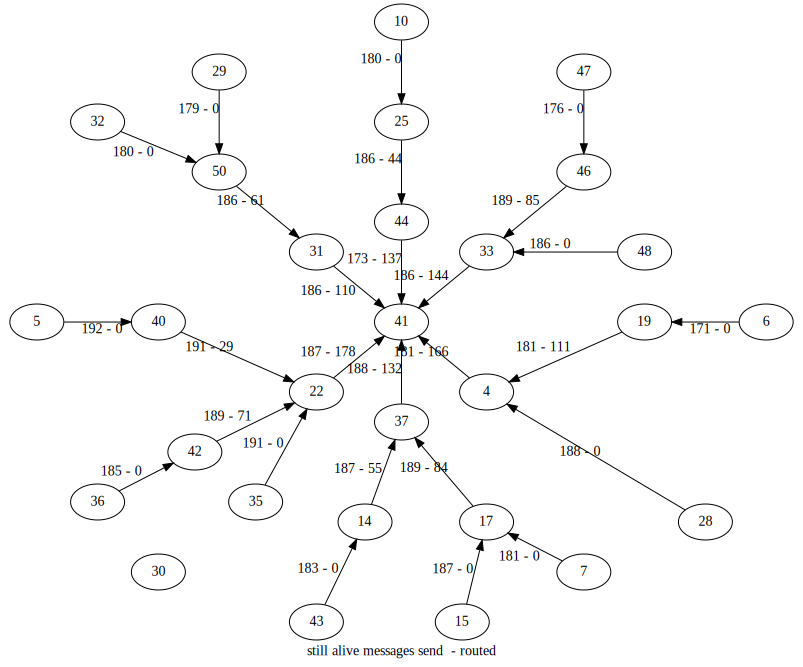
\includegraphics[width=1\textwidth]{images/messages.png}
     \caption{Experiment - počty zaslaných a přeposlaných zpráv}
     \label{img:msgs}
\end{figure}


První informace, kterou můžeme vidět je, že při práci s bezdrátovými sensorovými sítěmi je třeba počítat chybami. V případě provedeného experimentu se jedná o uzel s ID 30, který v průběhu celého experimentu 
nekomunikoval, tedy se pravděpodobně nepodařilo správně nainstalovat či inicializovat aplikaci na tomto konkrétním uzlu. Veškeré následují statistiky nezapočítávají tento uzel do výsledků, tedy celkový počet 
uzlů, který uvažujeme je 27 sensorových uzlů a jeden uzel centrální. 

Dále můžeme vidět, že maximální počet zpráv, které odeslal jeden uzel je $192$. Ze záznamů víme, že doba po kterou byly zprávy zachytávány  byla $939$ sekund a pokud počítáme jednu 
zprávu za $5$ sekund, vyjde nám předpokládaný počet odeslaných zpráv poněkud nižší, konkrétně $187$ zpráv. Obě hodnoty jsou však natolik blízké, že rozdíl lze zdůvodnit drobným rozdílem hodin na jednotlivých 
uzlech. Pokud tedy jako maximální počet zpráv, které uzel měl možnost odeslat určíme experimentálně zjištěnou hodnotu $192$, pak spočítáme, že se nám podařilo zachytit $96\%$ všech zpráv, 
které mohly být odeslány.

Zajímavější informace uvidíme, pokud se podíváme na jednotlivá procenta přeposlaných zpráv. Například uzlu s ID $50$ bylo určeno celkem 359 zpráv, které měl přeposlat, nicméně učinil tak pouze u 61 zpráv. 
Můžeme předpokládat, že zprávy které přijal, také přeposlal. Tedy můžeme dovodit, že uzel přijal pouze $17\%$ jemu určených zpráv. Pokud tuto statistiku spočítáme pro všechny uzly mimo okrajových, tyto žádné 
zprávy nepřeposílaly, zjistíme, že z celkového součtu zpráv určených k přeposlání bylo přeposláno pouze $32.4\%$ a jeden uzel průměrně přeposlal $36.9\%$. 

Procento přeposlaných zpráv je tedy překvapivě nízké. To že uzel nebyl schopen přijmout průměrně $64.5\%$ zpráv, které mu byly adresované lze vysvětlit tím, že při posílání zpráv není vyžadováno potvrzení o 
doručení a rušení způsobuje vysoké procento nedoručených zpráv. Rušení může být způsobeno jak ostatní komunikací v síti, tak vlivy vnějšího prostředí. Zde by tedy bylo vhodné zvážit dvě varianty řešení 
problému. Jednak je možné snížit komunikaci v síti pomocí prodloužení intervalů posílání jednotlivých zpráv a případně snížení dosahu rádiové komunikace tak, aby uzel měl možnost komunikovat pouze se 
sousedními uzly, tedy omezit rušení komunikace. Druhou variantou je změna typu zprávy tak, aby bylo vyžadováno potvrzení o doručení. Zde sice výrazně zvýšíme množství doručených zpráv, nicméně za cenu vyšší zátěže jednotlivých uzlů.


\subsection{IDS zprávy}

Druhá statistika \ref{img:reported} se zabývá systémem pro hlášení narušení sítě (IDS), kde jednotlivé uzly zaznamenávají aktivitu ostatních uzlů a pokud vyhodnotí, že některý z okolních uzlů zahazuje 
zprávy, které měl přeposlat, pak tento uzel nahlásí pomocí IDS zprávy. Tato statistika je zajímavá především v porovnání s předchozí statistikou přeposílání zpráv \ref{sub:alive}. Vzhledem k velmi vysokému 
procentu nepřeposlaných zpráv zde můžeme vidět velký počet IDS zpráv hlásících, že jednotlivé uzly zahazují zprávy. V našem případě se nejedná o úmyslné zahazování zpráv, ale toto IDS komponenta neumí 
rozlišit.

\begin{figure}[h]
     \centering
     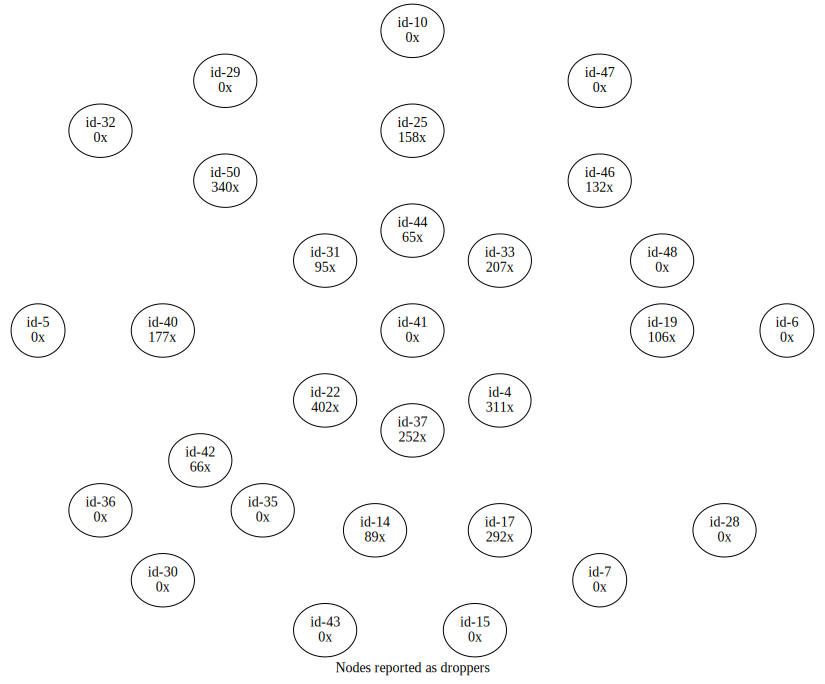
\includegraphics[width=1\textwidth]{images/idsReported.png}
     \caption{Experiment - statistika nahlášení jednotlivých uzlů pomocí IDS}
     \label{img:reported}
\end{figure}

Dle předpokladů můžeme vidět, že uzly umístěné na listech sítě nebyly ani jednou nahlášeny, protože nebyla žádná zpráva, kterou by měly přeposlat. Naopak všechny ostatní uzly nahlášeny 
byly a průměr nahlášení na jeden uzel je $183$ zpráv. 

V druhém grafu \ref{img:reporting} můžeme vidět, kolikrát který uzel poslal IDS zprávu, zde však nenalezneme překvapivý výsledek, počty zpráv jsou poměrně rovnoměrně rozděleny mezi všechny uzly v síti. 

Konkrétní porovnání hodnot přeposlaných zpráv a příslušný počet IDS zpráv pro konkrétní uzly je možné vidět v následující tabulce 
\ref{tab:ids}. Uzly umístěné na listech sítě nejsou do tabulky zahrnuty, protože jak 
bylo zmíněno dříve, tyto uzly nepřeposílaly žádné zprávy. 

\begin {table}[h]
\caption {počty přeposlaných zpráv a IDS hlášení pro konkrétní uzly} \label{tab:ids} 
\begin{center}
\begin{tabular}{rrrrr}

ID  & AliveExp &  AliveSend & $\frac{AliveSend}{AliveExp}$& IDS \\
\hline
4   &        480  &        166  &        34,58 \%  &        311 \\
14  &        183  &        55   &        30,05 \%  &        89  \\
17  &        368  &        84   &        22,83 \%  &        292 \\
19  &        171  &        111  &        64,91 \%  &        106 \\
22  &        671  &        132  &        19,67 \%  &        402 \\
25  &        180  &        44   &        24,44 \%  &        158 \\
31  &        247  &        137  &        55,47 \%  &        95 \\
33  &        460  &        144  &        31,30 \%  &        207 \\
37  &        515  &        166  &        32,23 \%  &        252 \\
40  &        192  &        29   &        15,10 \%  &        177 \\
42  &        185  &        71   &        38,38 \%  &        66 \\
44  &        230  &        144  &        62,61 \%  &        65 \\
46  &        176  &        85   &        48,30 \%  &        132 \\
50  &        359  &        61   &        16,99 \%  &        340 \\
\hline
\hline
součet &        4417 &        1429 &        32,4 \%   &        2692 \\
průměr &             &             &        35,5 \%  &        183 \\
\end{tabular}
\bigskip
\caption*{Zkratky použité pro pojmenování sloupců:\\
	  AliveExp -- očekávaný počet přeposlaných still-alive zpráv \\
	  AliveSend -- skutečný počet přeposlaných still-alive zpráv \\	  
	  IDS -- počet IDS nahlášení uzlu}
\end{center}
\end {table}

Celkově z IDS statistiky můžeme vidět, že detekce nepřeposílání zpráv funguje lépe, než samotné přeposílání. Tento fakt je pravděpodobně 
způsoben tím, že přeposlání zprávy má na starost pouze jeden uzel, zatímco detekovat nepřeposílání může kterýkoliv uzel v síti.
Protože víme, že velmi často docházelo k nepřeposílání zpráv \ref{sub:alive}, můžeme konstatovat, že IDS systém toto nepřeposílání správě
detekoval a tedy funguje tak, jak bylo zamýšleno.


\subsection{Zprávy detekce útočníka}

V průběhu experimentu došlo v oblasti monitorované sítí k pohybu útočníka. Tento byl z důvodu nedostatečné rozlišovací schopnosti sensorů 
pro detekci pohybu nahrazen uzlem vysílajícím zprávu, že se jedná o útočníka. Pokud uzly sítě přijmou zprávu vysílanou útočníkem, je tato 
skutečnost zaznamenána jako detekce pohybu útočníka. 

Zprávy o detekci útočníka byly zpracovány jednak pomocí statického grafu \ref{img:attacker}, který vyjadřuje kolik který uzel poslal 
zpráv o zaznamenání útočníka a jednak pomocí animace, která znázorňuje detekci pohybu útočníka v čase. 

Z grafu můžeme vidět, že detekce pohybu útočníka byla rozdílně úspěšná u jednotlivých uzlů, zatímco některé útočníka nezaznamenaly vůbec, 
tak jiné uzly zaznamenaly pohyb útočníka až šestkrát. Tento rozdíl je možné zdůvodnit pohybem útočníka, zatímco k některým uzlům se mohl 
uzel útočníka přiblížit na kratší vzdálenost či delší dobu, tak k jiným se nemusel přiblížit vůbec. Pohyb útočníka byl sice proveden 
po trase přibližně stejně vzdálené od všech uzlů v síti, nicméně k rozdílům mohlo dojít. Dále pokud se podíváme na statistiku doručení 
still-alive zpráv \ref{sub:alive} a předpokládáme stejnou úspěšnost doručení zpráv z uzlu útočníka, pak zcela jistě mohlo dojít k 
situaci, kdy část uzlů útočníka nezaznamenala vůbec. 

Lepší pohled na pohyb útočníka nám poskytne animace, kde můžeme pomocí změny barvy jednotlivých uzlů vidět, že odeslaly zprávu o 
detekování útočníka. Animace nám poskytuje data ve zpomalené podobě za účelem názornosti a lepší přehlednosti a jednotlivé zprávy 
o detekci útočníka jsou v animaci zobrazeny i po krátký časový interval po jejich odeslání tak, aby je bylo možné v animaci zaznamenat.

Celkově tedy můžeme vidět, jak jednotlivé uzly odesílají zprávy o detekci útočníka s tím, že tyto zprávy se objevují postupně a 
v oblastech, ve kterých se útočník pohyboval. Celkově lze tedy konstatovat, že systém detekce útočníka funguje, i když by bylo vhodné 
zvýšit množství zpráv indikujících přítomnost útočníka, což mimo jiné souvisí s již dříve diskutovaným problémem s doručováním zpráv. 

\subsection{Zprávy plošného vysílaní z centrálního uzlu}
Poslední skupina zpráv, která byla vyhodnocována, jsou zprávy vysílané z centrálního uzlu pomocí globálního broadcastu, určené všem uzlům 
v síti a slouží k přepnutí úrovně zabezpečení. U těchto zpráv nás zajímá jejich šíření v celé síti, protože tyto zprávy byly šířeny 
pomocí záplavy, tedy jakmile uzel zprávu obdrží, tak ji v původní podobě odvysílá, aby byla možnost rozšíření zprávy do všech oblastí 
sítě. V záznamech z průběhu experimentu máme možnost sledovat právě vysílání stejné zprávy z jednotlivých uzlů, tedy předpokládáme, že jakmile uzel zprávu 
odesílá, tak ji předtím v pořádku přijal.

Jediný rozumný způsob znázornění průběhu tohoto šíření zprávy v síti je animace postupného průběhu, protože statický graf by nám poskytl
u každého uzlu pouze logickou hodnotu, zdali přijal či nepřijal zprávu. Sice by šlo tento graf rozšířit o vhodné označení pořadí 
jednotlivých uzlů, nicméně i tak by byla orientace v grafu značně problematická. 

Díky animaci můžeme vidět, že původní záměr šíření zprávy postupnou záplavou od nejbližších uzlů po nejvzdálenější uzly zcela 
nefunguje. Můžeme totiž sledovat, že proces šíření zprávy je velmi chaotický a i když jednotlivé uzly reagují postupně, pak to zcela 
jistě není v námi zamýšleném pořadí. Z toho je tedy možné dovodit, stejně jako v předchozích případech, že úspěšnost doručení zpráv je 
velmi malá a taktéž to, že vysílací výkon jednotlivých uzlů nezahrnuje pouze nejbližší sousedy, ale i například uzly na opačné polovině 
sítě. 

Celkově se vždy podařilo zaznamenat doručení zprávy na většinu uzlů (pravděpodobně se zprávu podařilo doručit na všechny uzly, jelikož 
všechny uzly dále vysílají na odpovídajícím stupni zabezpečení), ale zjistili jsme, že způsob šíření zprávy je velmi chaotický, především
kvůli nepředpokládaně vysokému vysílacímu výkonu jednotlivých uzlů a taktéž kvůli nízké úspěšnosti doručování jednotlivých zpráv.

\chapter{Závěr}

V práci jsem se zabýval problémem distribuce klíčů v bezdrátových sensorových sítích. V první kapitole jsem nejdříve uvedl důvody, proč není vhodné používat klasická řešení distribuce klíčů
a následně jsem rozebral několik různých návrhů optimalizovaných pro bezdrátové sensorové sítě. U každého z nich jsem postupně uvedl základní principy a následně krátké zhodnocení výhod a nevýhod konkrétního 
návrhu včetně vyhodnocení vhodnosti použití schématu při implementaci vyvíjené komponenty. 

Následující kapitola se zabývá samotnou implementací schématu LEAP+. Nejdříve je krátce uveden použitý operační systém TinyOS a specifické problémy při psaní aplikace pro tento systém. Následuje podrobný 
popis předpokládaných vlastností vyvíjené komponenty společně s důvody pro výběr LEAP+ schématu. Dále jsou zde rozvedeny a odůvodněny odlišnosti v implementaci oproti původnímu návrhu. Poslední část kapitoly 
tvoří krátký popis implementace samotné. 

Třetí kapitola je zaměřena na experiment Mírov 2014, postupně je popsán průběh experimentu a programy použité pro vyhodnocení. Kapitola končí samotným vyhodnocením, jsou rozebrány jednotlivé typy zachycených 
zpráv a získaná data jsou interpretována. 

Jak vyplynulo z dat získaných při experimentu, celá experimentální platforma ProtectLayer funguje, nicméně pro optimální výkon celé sítě by bylo potřeba provést několik změn. Především by komunikaci v síti 
velmi pomohlo snížení dosahu rádiové komunikace tak, aby uzel měl možnost kontaktovat pouze nejbližší sousedy. I když se tato skutečnost může zdát přesně tím opačným řešením, které by se nabízelo, ve 
skutečnosti snížení dosahu komunikace sníží vytížení jednotlivých uzlů a tím pravděpodobně zvýší pravděpodobnost doručení zpráv. Tuto úpravu by ještě bylo možné vylepšit, pokud by intervaly posílání 
jednotlivých zpráv byly prodlouženy. Druhou variantou zlepšení výkonu je vyžadování potvrzení o přijetí odeslaných zpráv.

Z hlediska možností navázání na tuto práci, konkrétně co se týká rozšíření současné podoby implementace o další funkcionalitu, moc prostoru nenaskýtá, protože při experimentu se jednotlivé uzly pohybovaly 
na hranici svých možností, především z hlediska dostupné paměti. Na druhou stranu je zcela jistě možné hledat jiné přístupy k řešení problému distribuce klíčů a například 
optimalizovat celou komponentu vzhledem k paměťové kapacitě jednotlivých uzlů.
Dále se nabízí spousta příležitostí pro další práci v oblasti vyhodnocení získaných dat, kde je zcela určitě možné vyvinuté nástroje rozšířit 
tak, aby poskytovaly celou řadu dalších statistik, případně aby program samotný umožňoval propojení různých statistik dohromady a tak usnadnil hledání závislostí.


\appendix

\chapter{Přílohy}


\section{TinyOS -- formát zpráv} \label{sec:msg}

V případě, že použijeme standardní variantu posílání zpráv v systému TinyOS, setkáme se u zachycených zpráv s následujícím formátem hlavičky \cite{TinyOSmsgs}.

\begin{verbatim}
00  ff ff  00 10  04  22  06
\end{verbatim}

První byte (00) určuje, že se jedná o AM paket\footnote{active message -- formát zprávy využívaný v TinyOS k událostmi řízenému modelu zpracování přijatých zpráv.}
Následující dva byty (ff~ff) určují adresu příjemce zprávy, v tomto případě zde můžeme vidět maximální možnou hodnotu, tedy se jedná o zprávu určenou všem uzlům.
Poté je uvedena adresa odesílajícího uzlu (00~10), tedy tato zpráva byla odeslána uzlem s ID 16 (hodnoty jsou uváděny v hexadecimální podobě). Další pole (04) určuje délku zprávy
a poslední dvě hodnoty (22~06) jsou postupně skupinové ID a poté ID komponenty navázané na tento typ zprávy (handler~ID). Skupinové ID slouží k tomu, aby na stejném kanálu bylo možné provozovat více
skupin uzlů bez vzájemného rušení. Handler~ID je využito v modelu událostmi řízeného zpracování přijatých zpráv tak, že zpráva je předána komponentě, jejíž ID zpráva obsahuje. 


\section{Skript pro vytvoření animace}\label{sec:script}
\begin{lstlisting}[ language=sh]
#!/bin/bash
for file in *.dot; do dot -Kneato -n -Tpng "$file" -o\
"$(basename $file .dot).png"; done

for file in *.png; do convert\
"$file" "$(basename $file .png).gif"; done

gifsicle --delay=1 --loop *.gif > anim.gif

\end{lstlisting}


\chapter{Doplňující materiály k experimentu}

\section{Rozmístění uzlů během experimentu}
\begin{figure}[h]
     \centering
     \includegraphics[width=1\textwidth]{images/scenario.png}
     \captionsource{Experiment - rozmístění uzlů}{\cite{Svenda2014}}
     \label{img:scenario}
\end{figure}

\newpage
\section{Statistika IDS hlášení poslaných jednotlivými uzly }
\begin{figure}[h]
     \centering
     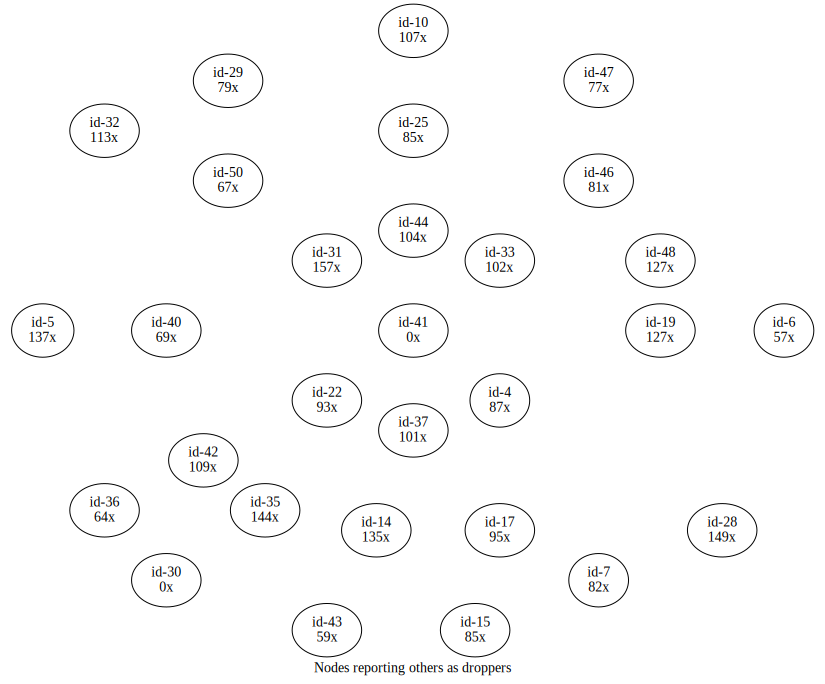
\includegraphics[width=1\textwidth]{images/idsReporting.png}
     \caption{Experiment - statistika IDS hlášení poslaných jednotlivými uzly}
     \label{img:reporting}
\end{figure}

\newpage
\section{Počet hlášení o pohybu útočníka u jednotlivých uzlů}
\begin{figure}[h]
     \centering
     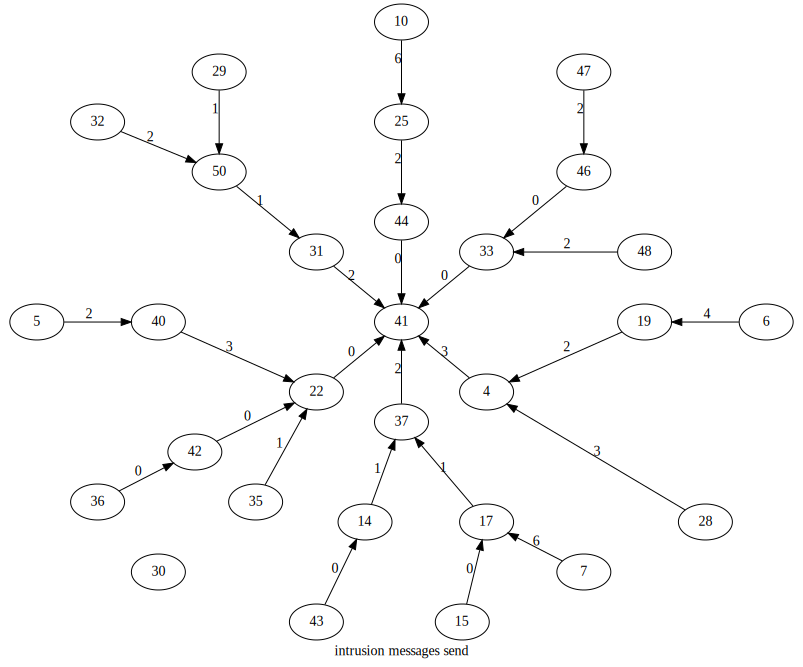
\includegraphics[width=1\textwidth]{images/attackerSum.png}
     \caption{Experiment - statistika hlášení o pohybu útočníka u jednotlivých uzlů}
     \label{img:attacker}
\end{figure}



%% Lists of tables and figures, glossary, etc.
%\printindex
%\printglossary
%\listoffigures
%\listoftables
%% Bibliography from lib.bib
\begingroup
\def\tmpchapter{0}
\renewcommand{\chaptername}{}
\renewcommand{\thechapter}{}
\addtocontents{toc}{\setcounter{tocdepth}{-1}}
\chapter{Literatura}
\renewcommand{\chapter}[2]{}% for other classes

\bibliographystyle{plain}
\bibliography{lib.bib}

\addtocontents{toc}{\setcounter{tocdepth}{2}}
\endgroup

%% Additional materials


%% End of the whole document
\end{document}